%%%%%%%%%%%%%%%%%%%%%%%%%%%%%%%%%%%%%%%%%%%%%%%%%%%%%%%%%%%%%%%%%%%%%%%%
%% Customizações do abnTeX2                                            %%
%% para a Universidade de Fortaleza                                   %%
%%%%%%%%%%%%%%%%%%%%%%%%%%%%%%%%%%%%%%%%%%%%%%%%%%%%%%%%%%%%%%%%%%%%%%%%

% !TEX root = ../main.tex
%%%%%%%%%%%%%%%%%%%%%%%%%%%%%%%%%%%%%%%%%%%%%%%%%%%%%%%%%%%%%%%%%%%%%%%%
%% Customizações do abnTeX2 (http://abnTeX2.googlecode.com)           %%
%% para a Universidade de Fortaleza						              %%
%%                                                                    %%
%% This work may be distributed and/or modified under the             %%
%% conditions of the LaTeX Project Public License, either version 1.3 %%
%% of this license or (at your option) any later version.             %%
%% The latest version of this license is in                           %%
%%   http://www.latex-project.org/lppl.txt                            %%
%% and version 1.3 or later is part of all distributions of LaTeX     %%
%% version 2005/12/01 or later.                                       %%
%%                                                                    %%
%% This work has the LPPL maintenance status `maintained'.            %%
%%                                                                    %%
%% The Current Maintainer of this work is Bruno Lopes                 %%
%%                                                                    %%
%% Project available on: https://github.com/bruno-unifor/unifortex2   %%
%%                                                                    %%
%% Further information about abnTeX2                                  %%
%% are available on http://abntex2.googlecode.com/                    %%
%%                                                                    %%
%%%%%%%%%%%%%%%%%%%%%%%%%%%%%%%%%%%%%%%%%%%%%%%%%%%%%%%%%%%%%%%%%%%%%%%%

\documentclass[
    a4paper,          % Tamanho da folha A4
    12pt,             % Tamanho da fonte 12pt
    chapter=TITLE,    % Todos os capitulos devem ter caixa alta
    section=TITLE,    % Todas as secoes devem ter caixa alta
    oneside,          % Usada para impressao em apenas uma face do papel
    english,          % Hifenizacoes em ingles
    spanish,          % Hifenizacoes em espanhol
    brazil            % Ultimo idioma eh o idioma padrao do documento
]{abntex2}

% Importações de pacotes
\usepackage[brazil]{babel} 
\usepackage[utf8]{inputenc}                         % Acentuação direta
\usepackage[T1]{fontenc}                            % Codificação da fonte em 8 bits
\usepackage{graphicx}                               % Inserir figuras
\usepackage{amsfonts, amssymb, amsmath}             % Fonte e símbolos matemáticos
\usepackage{booktabs}                               % Comandos para tabelas
\usepackage{verbatim}                               % Texto é interpretado como escrito no documento
\usepackage{multirow, array}                        % Múltiplas linhas e colunas em tabelas
\usepackage{indentfirst}                            % Endenta o primeiro parágrafo de cada seção.
\usepackage{listings}                               % Utilizar codigo fonte no documento
\usepackage{xcolor}
\usepackage{microtype}                              % Para melhorias de justificação?
\usepackage[portuguese,ruled,lined]{algorithm2e}    % Escrever algoritmos
\usepackage{algorithmic}                            % Criar Algoritmos
%\usepackage{float}                                  % Utilizado para criação de floats
\usepackage{amsgen}
\usepackage{lipsum}                                 % Usar a simulação de texto Lorem Ipsum
%\usepackage{titlesec}                               % Permite alterar os títulos do documento
\usepackage{tocloft}                                % Permite alterar a formatação do Sumário
\usepackage{etoolbox}                               % Usado para alterar a fonte da Section no Sumário
\usepackage[nogroupskip,nonumberlist,acronym]{glossaries}                % Permite fazer o glossario
\usepackage{caption}                                % Altera o comportamento da tag caption
\usepackage[alf, abnt-emphasize=bf, bibjustif, recuo=0cm, abnt-etal-cite=3, abnt-etal-list=0,abnt-etal-text=it]{abntex2cite}  % Citações padrão ABNT
%\usepackage[bottom]{footmisc}                      % Mantém as notas de rodapé sempre na mesma posição
%\usepackage{times}                                 % Usa a fonte Times
\usepackage{mathptmx}                               % Usa a fonte Times New Roman
%\usepackage{lmodern}                               % Usa a fonte Latin Modern
%\usepackage{subfig}                                % Posicionamento de figuras
%\usepackage{scalefnt}                              % Permite redimensionar tamanho da fonte
%\usepackage{color, colortbl}                       % Comandos de cores
%\usepackage{lscape}                                % Permite páginas em modo "paisagem"
%\usepackage{ae, aecompl}                           % Fontes de alta qualidade
%\usepackage{picinpar}                              % Dispor imagens em parágrafos
%\usepackage{latexsym}                              % Símbolos matemáticos
%\usepackage{upgreek}                               % Fonte letras gregas
\usepackage{appendix}                               % Gerar o apendice no final do documento
\usepackage{paracol}                                % Criar paragrafos sem identacao
\usepackage{lib/unifortex2}		                    % Biblioteca com as normas da Unifor para trabalhos academicos
\usepackage{pdfpages}                               % Incluir pdf no documento
\usepackage{amsmath}                                % Usar equacoes matematicas

% Organiza e gera a lista de abreviaturas, simbolos e glossario
\makeglossaries

% Gera o Indice do documento
\makeindex


%%%%%%%%%%%%%%%%%%%%%%%%%%%%%%%%%%%%%%%%%%%%%%%%%%%%%
%%         Configuracoes do uniforTeX2             %%
%%%%%%%%%%%%%%%%%%%%%%%%%%%%%%%%%%%%%%%%%%%%%%%%%%%%%

%\trabalhoacademico{tccgraduacaoPDF}
\trabalhoacademico{tccgraduacao}
%\trabalhoacademico{tccespecializacao}
%\trabalhoacademico{dissertacao}
%\trabalhoacademico{tese}

\ehqualificacao{nao}

\removerbordasdohyperlink{sim}

\cordohyperlink{nao}

%%%%%%%%%%%%%%%%%%%%%%%%%%%%%%%%%%%%%%%%%%%%%%%%%%%%%
%%         Informação sobre a IES                  %%
%%%%%%%%%%%%%%%%%%%%%%%%%%%%%%%%%%%%%%%%%%%%%%%%%%%%%

\ies{Universidade de Fortaleza}
\iessigla{UNIFOR}
\centro{Centro de Ciências Tecnológicas}

%%%%%%%%%%%%%%%%%%%%%%%%%%%%%%%%%%%%%%%%%%%%%%%%%%%%%
%%         Informação para TCC de Graduacao        %%
%%%%%%%%%%%%%%%%%%%%%%%%%%%%%%%%%%%%%%%%%%%%%%%%%%%%%

\graduacaoem{Ciência da Computação}
\habilitacao{bacharel}

%%%%%%%%%%%%%%%%%%%%%%%%%%%%%%%%%%%%%%%%%%%%%%%%%%%%%
%%     Informação para TCC de Especializacao       %%
%%%%%%%%%%%%%%%%%%%%%%%%%%%%%%%%%%%%%%%%%%%%%%%%%%%%%

\especializacaoem{}

%%%%%%%%%%%%%%%%%%%%%%%%%%%%%%%%%%%%%%%%%%%%%%%%%%%%%
%%         Informação para Dissertacao             %%
%%%%%%%%%%%%%%%%%%%%%%%%%%%%%%%%%%%%%%%%%%%%%%%%%%%%%

%\programamestrado{Programa de Pós-Graduação em Informática Aplicada}
%\nomedomestrado{Mestrado Acadêmico em Ciência da Computação}
%\mestreem{Ciência da Computação}
%\areadeconcentracaomestrado{Ciência da Computação}

%%%%%%%%%%%%%%%%%%%%%%%%%%%%%%%%%%%%%%%%%%%%%%%%%%%%%
%%                 Informação para Tese            %%
%%%%%%%%%%%%%%%%%%%%%%%%%%%%%%%%%%%%%%%%%%%%%%%%%%%%%

%\programadoutorado{Programa de Pós-Graduação em Informática Aplicada}
%\nomedodoutorado{Doutorado em Saúde Coletiva}
%\doutorem{Saúde Coletiva}
%\areadeconcentracaodoutorado{Saúde Coletiva}

%%%%%%%%%%%%%%%%%%%%%%%%%%%%%%%%%%%%%%%%%%%%%%
%%  Informação relacionadas a trabalhos     %%
%%%%%%%%%%%%%%%%%%%%%%%%%%%%%%%%%%%%%%%%%%%%%%

\autor{João Felipe Ribeiro de Melo \\ João Pedro Ribeiro Mendes}

\titulo{
ARQUITETURA DE SISTEMAS OFFLINE-FIRST COMO AMPARO À PRÁTICA
VETERINÁRIA EM REGIÕES DE BAIXA CONECTIVIDADE.
}

\data{2026}

\local{Fortaleza -- Ceará}

%\dataaprovacao{01 de Janeiro de 2017}

%%%%%%%%%%%%%%%%%%%%%%%%%%%%%%%%%%%%%%%%%%%%%
%%     Informação sobre o Orientador       %%
%%%%%%%%%%%%%%%%%%%%%%%%%%%%%%%%%%%%%%%%%%%%%

\orientador{Belmondo Rodrigues Aragão Júnior}
%\orientadories{Universidade de Fortaleza - UNIFOR}
%\orientadorcentro{Centro de Ciências Tecnológicas - CCT}
%\orientadorfeminino{nao}

%%%%%%%%%%%%%%%%%%%%%%%%%%%%%%%%%%%%%%%%%%%%%
%%      Informação sobre o Co-orientador   %%
%%%%%%%%%%%%%%%%%%%%%%%%%%%%%%%%%%%%%%%%%%%%%

%\coorientador{}
%\coorientadories{Universidade Co-orientador - SIGLA}
%\coorientadorcentro{Centro do Co-orientador - SIGLA}
%\coorientadorfeminino{nao}

%%%%%%%%%%%%%%%%%%%%%%%%%%%%%%%%%%%%%%%%%%%%%
%%      Informação sobre a banca           %%
%%%%%%%%%%%%%%%%%%%%%%%%%%%%%%%%%%%%%%%%%%%%%

%\membrodabancadois{Membro da Banca Dois}
%\membrodabancadoiscentro{Centro de Ciências e Tecnologia - CCT}
%\membrodabancadoisies{Universidade do Membro da Banca Dois - SIGLA}

%\membrodabancatres{Membro da Banca Três}
%\membrodabancatrescentro{Centro de Ciências e Tecnologia - CCT}
%\membrodabancatresies{Universidade do Membro da Banca Três - SIGLA}

%\membrodabancaquatro{Membro da Banca Quatro}
%\membrodabancaquatrocentro{Centro de Ciências e Tecnologia - CCT}
%\membrodabancaquatroies{Universidade do Membro da Banca Quatro - SIGLA}

%\membrodabancacinco{Membro da Banca Cinco}
%\membrodabancacincocentro{Centro de Ciências e Tecnologia - CCT}
%\membrodabancacincoies{Universidade do Membro da Banca Cinco - SIGLA}

%\membrodabancaseis{Membro da Banca Seis}
%\membrodabancaseiscentro{Centro de Ciências e Tecnologia - CCT}
%\membrodabancaseisies{Universidade do Membro da Banca Seis - SIGLA}

\usepackage{float}
% NBR 6023:2018: os endereços eletrônicos não são mais delimitados por < >.
% O abntex2cite ainda os adiciona; aqui eles são removidos.
\makeatletter\def\UrlLeft{}\def\UrlRight{}\makeatother

\makeatletter
\renewcommand{\folhaderostocontent}{%
    \begin{center}
        \normalsize
        \MakeUppercase{\imprimirautor}\par
        \vspace{6.5cm}
        \MakeUppercase{\imprimirtitulo}\par
    \end{center}

    \vspace{2.5cm}

    \noindent
    \hspace*{6cm}%
    \begin{minipage}{8cm}
        \begin{SingleSpace}
            \imprimirpreambulo\par
            \medskip

            \abntex@ifnotempty{\imprimirorientador}{%
                \noindent
                \artigoorientador:
                \imprimirorientador\par
            }

            \abntex@ifnotempty{\imprimircoorientador}{%
                \noindent
                \artigocoorientador:
                \imprimircoorientador\par
            }
        \end{SingleSpace}
    \end{minipage}

    \vfill

    \begin{center}
        \normalsize
        \MakeUppercase{\imprimirlocal}\par
        \imprimirdata\par
    \end{center}
}
\makeatother

\begin{document}

    %%%%%%%%%%%%%%%%%%%%%%%%%%%%%%%%%%%%%%%%%%%%%%%%%%%%%%%%%%%%%%%%%%%%%%%
    %% Elementos pré-textuais                                            %%
    %%%%%%%%%%%%%%%%%%%%%%%%%%%%%%%%%%%%%%%%%%%%%%%%%%%%%%%%%%%%%%%%%%%%%%%
    
    \imprimircapa
    \begin{folhaderosto}
        \folhaderostocontent
    \end{folhaderosto}    % Ficha catalográfica inserida como PDF%
    %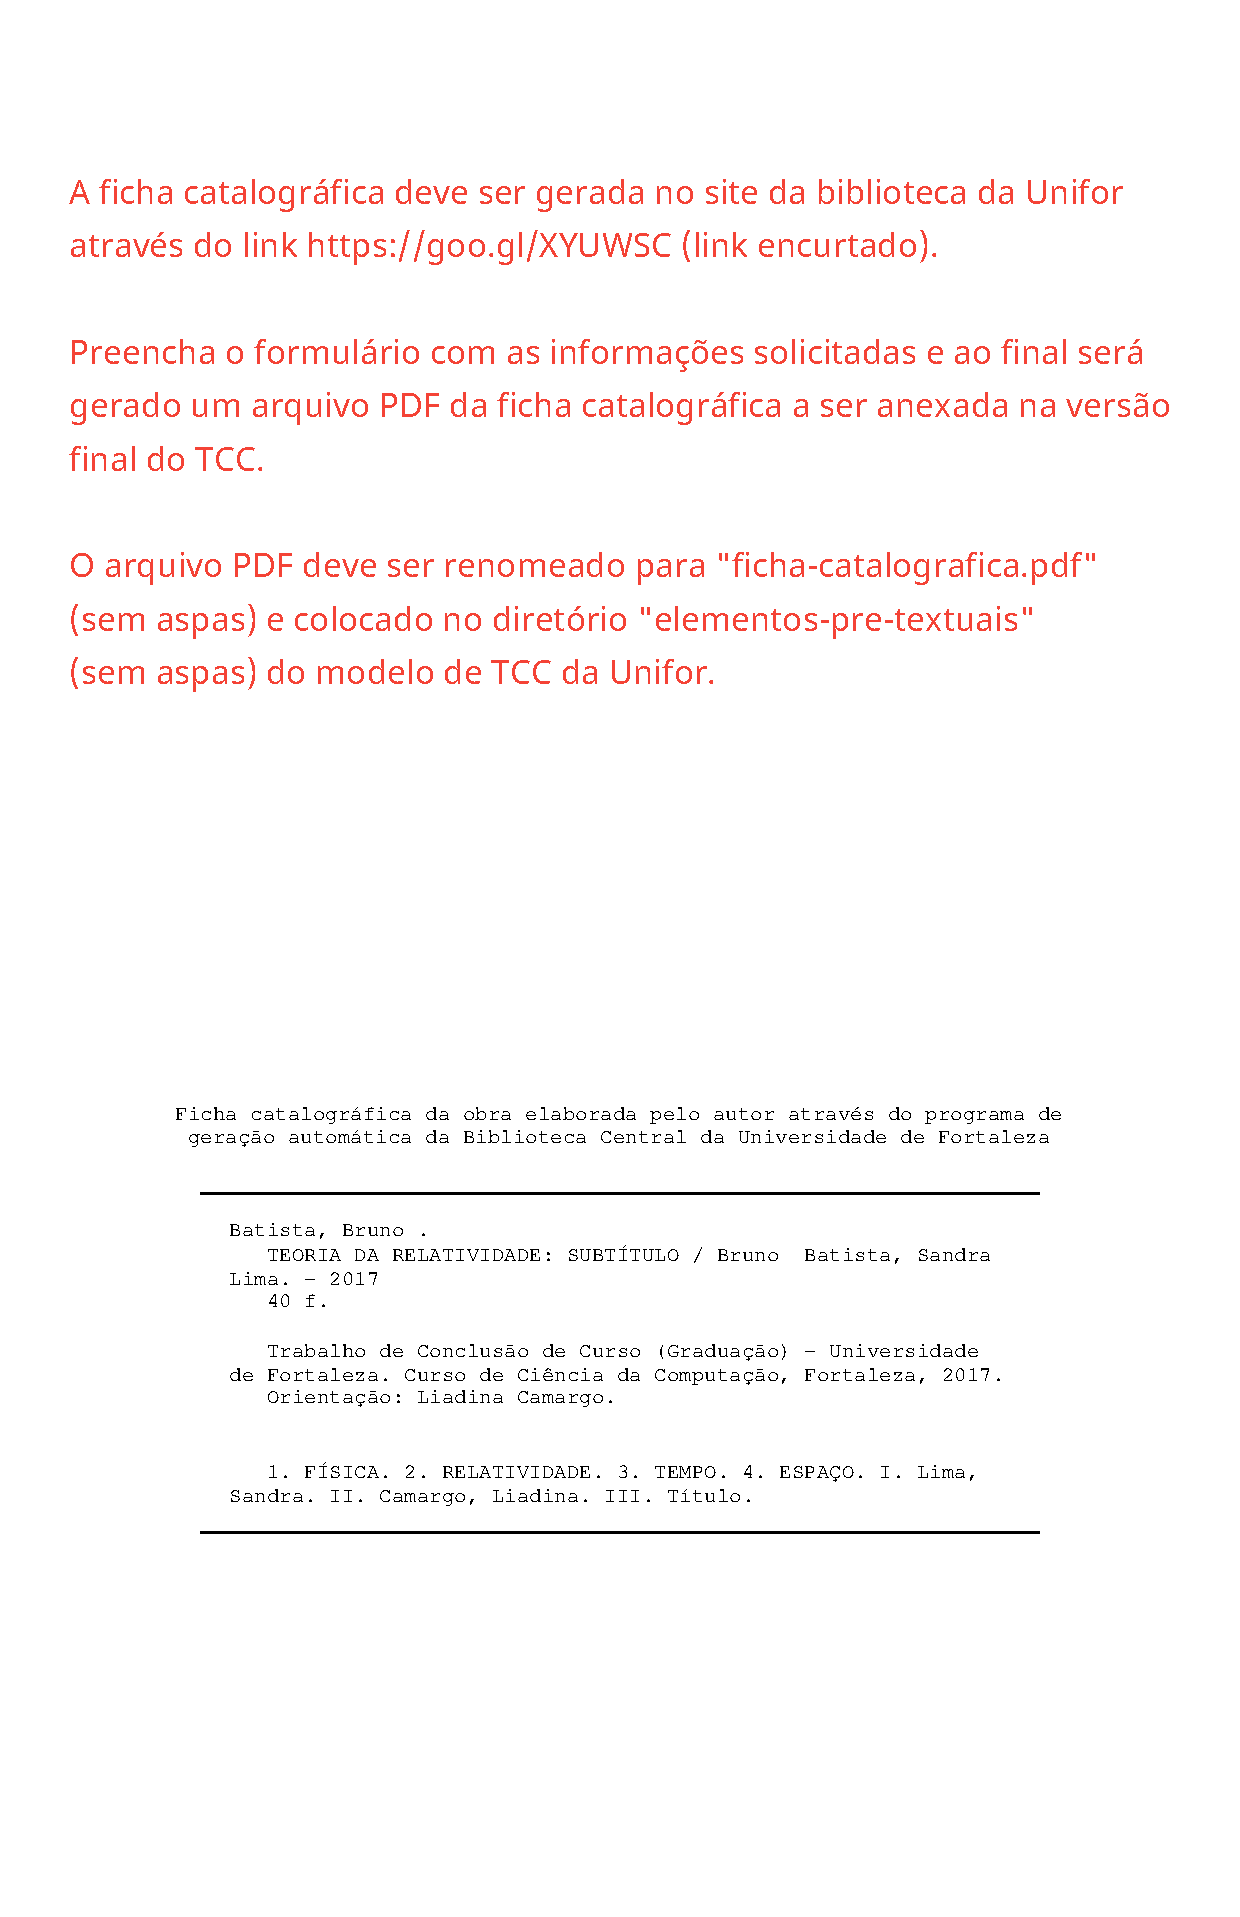
\includepdf{elementos-pre-textuais/ficha-catalografica.pdf}%
    % Errata incluída via arquivo .tex%
    %\begin{errata}
\end{errata}

    % Folha de aprovação inserida como PDF}
    %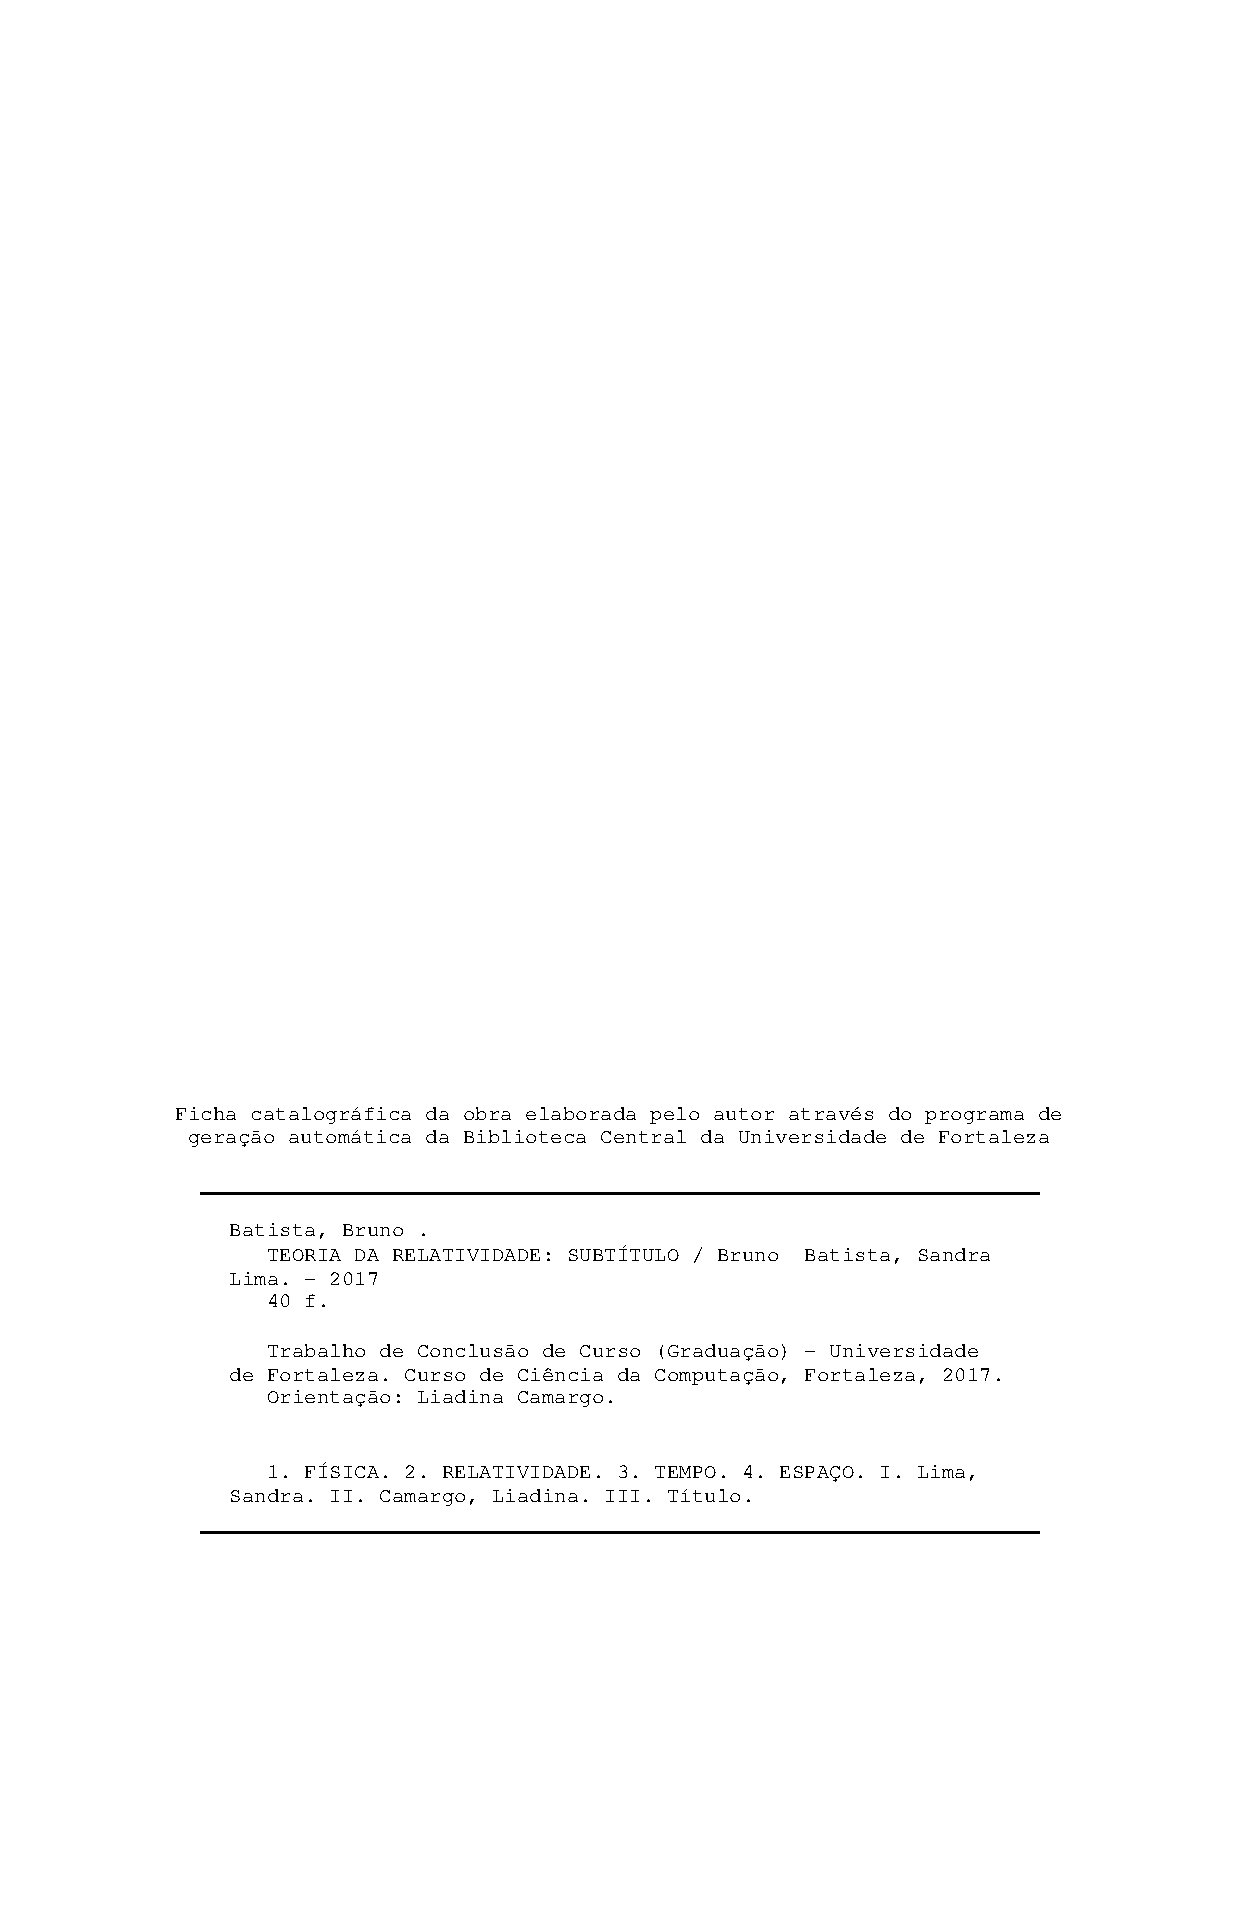
\includepdf{elementos-pre-textuais/folha-aprovacao.pdf}
    
    %\imprimirdedicatoria{elementos-pre-textuais/dedicatoria}
    %\imprimiragradecimentos{elementos-pre-textuais/agradecimentos}
    %\imprimirepigrafe{elementos-pre-textuais/epigrafe}
    \imprimirresumo{elementos-pre-textuais/resumo}
    \imprimirabstract{elementos-pre-textuais/abstract}
    \imprimirlistadeilustracoes
    \clearpage % a classe não quebra a página após a lista de ilustrações
    % \imprimirlistadetabelas da classe gera uma página em branco antes da lista de siglas;
    % por isso a lista de tabelas é impressa diretamente (a lista de siglas já inicia nova página).
    \begin{KeepFromToc}\listoftables\end{KeepFromToc}
    %\imprimirlistadequadros
    %\imprimirlistadealgoritmos
    %\imprimirlistadecodigosfonte
    \glsaddall[types={\acronymtype}]
    \imprimirlistadeabreviaturasesiglas
    %\imprimirlistadesimbolos{elementos-pre-textuais/lista-de-simbolos} % Comentado temporariamente para evitar erro de lista vazia
    \imprimirsumario

    %%%%%%%%%%%%%%%%%%%%%%%%%%%%%%%%%%%%%%%%%%%%%%%%%%%%%%%%%%%%%%%%%%%%%%%
    %% Elementos textuais                                                %%
    %%%%%%%%%%%%%%%%%%%%%%%%%%%%%%%%%%%%%%%%%%%%%%%%%%%%%%%%%%%%%%%%%%%%%%%
    \textual

    \chapter{Introdução}
\label{cap:introducao}

% Os algoritmos de aprendizado de máquina que fazem classificação em imagens, necessitam que estas sejam de baixa dimensionalidade \cite{yang2019re} . \gls{KNN} askjdhkjasdhj ashdkajsdhajkhj \gls{KNN}

No cenário contemporâneo de digitalização dos serviços, o setor médico-veterinário enfrenta o desafio de transpor a eficiência clínica para o ambiente domiciliar. Essa transição é impulsionada não apenas pela demanda por conveniência, mas sobretudo pelo bem-estar animal. Ao analisar o comportamento felino, observou-se que "os gatos apresentaram níveis de estresse significativamente menores quando examinados em um ambiente doméstico em comparação com um ambiente clínico", (Nibblett, 2015). Diante disso, torna-se imperativo o desenvolvimento de ferramentas robustas voltadas especificamente para a gestão do atendimento remoto e volante.

Tendo isso em vista, médicos veterinários que atuam em atendimentos domiciliares enfrentam desafios acentuados que comprometem a agilidade e a segurança do serviço. A dependência de conectividade constante cria uma barreira crítica: em localidades com infraestrutura de rede deficitária, o uso de sistemas baseados exclusivamente na presença de internet e nuvem, frequentemente inviabiliza o fluxo ideal, forçando o veterinário a recorrer a registros improvisados em papel ou na memória. Estudos na área de informática em saúde apontam que essa fragmentação da informação eleva significativamente o risco de perda de dados, problemas de legibilidade e erros de transcrição posterior (F.L Pollari, 1996). Além das falhas operacionais, essa dinâmica impede o acesso imediato ao histórico clínico completo do paciente no local de atendimento, momento crucial do exame clínico no qual a tomada de decisão exige rapidez e fundamentação baseada em evidências (Kristine M. Alpi, 2011).

De que foram uma arquitetura \textit{offline-first} pode contribuir para a sincronização de dados clínico-veterinários em contextos de baixa conectividade? Diante desse problema, é necessária a investigação de técnicas que contribuam com o armazenamento de dados de uma aplicação veterinária, de forma que, sem a presença de internet no dispositivo móvel do usuário, os dados sejam persistidos primeiramente na camada local e, posteriormente, no servidor. Para alcançar esse objetivo, o seguinte trabalho apresenta o desenvolvimento do RoadVet, uma aplicação móvel voltada para médicos veterinários autônomos que atuam em atendimento domiciliar, baseada na arquitetura \textit{offline-first}, arquitetura que prioriza o uso da aplicação no dispositivo do usuário, buscando que os dados sejam salvos primordialmente na camada de apresentação, que no presente trabalho é implementada com a tecnologia \textit{React Native} para a interface do usuário e a biblioteca \textit{WatermelonDB}, responsável por persistir esses dados no dispositivo do veterinário, quando a conexão com a internet é identificada, os dados que foram criados são sincronizados com a camada de suporte, que foi abstraída como uma API(\textit{Application Programming Interface}), construída utilizando o\textit{ Django Rest Framework} e um banco de dados relacional\textit{ SQLite}, para manter as informações acessíveis.

Além desta introdução, o presente documento está estruturado da seguinte maneira: o Capítulo ~\ref{cap:fundamentacao-teorica} trata da fundamentação teórica, abordando o mercado de cuidado animal e o meio social, o paradigma \textit{offline-first} e a legislação que apoia esses animais de estimação. O capítulo ~\ref{cap:trabalhos-relacionados} traz os trabalhos relacionados que serviram como exemplo para o desenvolvimento do RoadVet. O capítulo ~\ref{chap:metodologia} destaca a metodologia adotada, que envolve a caracterização da pesquisa, discussão com profissionais da área veterinária, processo de levantamento de requisitos, com alguns exemplos, definição da arquitetura da aplicação que foi desenvolvida e o procedimento de validação e testes adotados. O capítulo ~\ref{cap:roadvet} trata do detalhamento do desenvolvimento do RoadVet, demonstrando visualmente o fluxo da aplicação, entre\textit{ back-end} e \textit{front-end}, uma visão geral do aplicativo móvel e a especificação do fluxo de uso principal do RoadVet. O capítulo ~\ref{cap:conclusao} debate as conclusões, dificuldades encontradas e os trabalhos futuros.

% \ref{fig:fluxogramaDeAlgumaCoisa}. 

% \ref{fig:oficial}

\section{Motivação}
\label{sec:motivacao}

Neste contexto, percebe-se que o uso de ferramentas tecnológicas que não dependam de acesso a Internet podem ajudar o trabalho de um veterinário domiciliar. Ao desenvolver uma solução que funcione de maneira \textit{offline}, busca-se otimizar o tempo desses profissionais, ao mesmo tempo que oferecer um serviço que aumente a eficiência e qualidade do cuidado animal, permitindo que o foco permaneça no atendimento e não nas limitações tecnológicas do local.

Este desenvolvimento estabelece, ainda, o alicerce necessário para futuras expansões modulares, como a otimização logística de deslocamentos.

\section{Objetivos}
\label{sec:objetivos}

Este trabalho tem como objetivo abordar o tema proposto e identificar as principais necessidades de médicos veterinários. A seguir, são apresentados os objetivos geral e específicos que norteiam este trabalho.

\subsection{Objetivo Geral}
\label{sec:objetivo-geral}

Desenvolver uma aplicação móvel voltada para atendimentos médico-veterinários domiciliares, utilizando uma arquitetura \textit{offline-first} capaz de persistir localmente e sincronizar no servidor, os dados, mesmo em ambientes de baixa conexão com a internet.

\subsection{Objetivos Específicos}
\label{sec:objetivos-especificos}

Os objetivos específicos do presente trabalho consistem na implementação da estratégia \textit{offline-first}, que foca na persistência de dados, partindo da camada do cliente. Essa abordagem visa garantir que os dados inseridos pelo usuário sejam sincronizados no servidor. Para tanto definem-se os seguintes passos: 

	\begin{itemize}
     \renewcommand\labelitemi{-}
		\item Analisar e implementar tecnologias existentes que sejam capazes de persistir os dados localmente, em dispositivos móveis.
		\item Implementar tecnologia de armazenamento local na camada do usuário, de forma que sejam visíveis os dados que ainda não foram sincronizados com o servidor.
        \item Projetar mecanismo de sincronização assíncrona.
		\item Realizar simulação de testes clínicos reais, de forma que o usuário final tenha uma arquitetura segura.
	\end{itemize}
    \chapter{Fundamentação Teórica}
\label{cap:fundamentacao-teorica}

%CORRIGIDO
Este capítulo apresenta a fundamentação teórica que embasa este projeto de conclusão de curso. Inicialmente, discute-se o crescimento do cuidado animal, em seguida, o paradigma \textit{offline-first} e, por fim, os aspectos de segurança e proteção de dados.

%CORRIGIDO
\section{Cuidado Animal}
%CORRIGIDO
Atualmente, percebe-se um crescimento da população de animais de estimação e a mudança nos perfis familiares, nos quais os \textit{pets} ocupam o patamar de membros da família. Isso tem impulsionado a demanda por serviços médico-veterinários mais ágeis, especializados e descentralizados. Dados do setor indicam que o Brasil encerrou o ano de 2023 com aproximadamente 160,9 milhões de animais de estimação, ocupando a terceira posição mundial em população \textit{pet}, o que intensifica a necessidade de assistência clínica constante \cite[p.~6]{abinpet2024}. Esse cenário de forte apelo afetivo e econômico estimula a expansão de novas modalidades de prestação de serviços, com destaque para o atendimento clínico domiciliar. A Figura~\ref{fig:graficopetsmundo}, elaborada com dados da consultoria GfK, ilustra a posição do Brasil na população mundial de animais de estimação.

\begin{figure}[H] 
    \centering 
    %CORRIGIDO
    \caption{Posição do Brasil na População Mundial de Animais de Estimação (2023)} 
    \label{fig:graficopetsmundo} 
    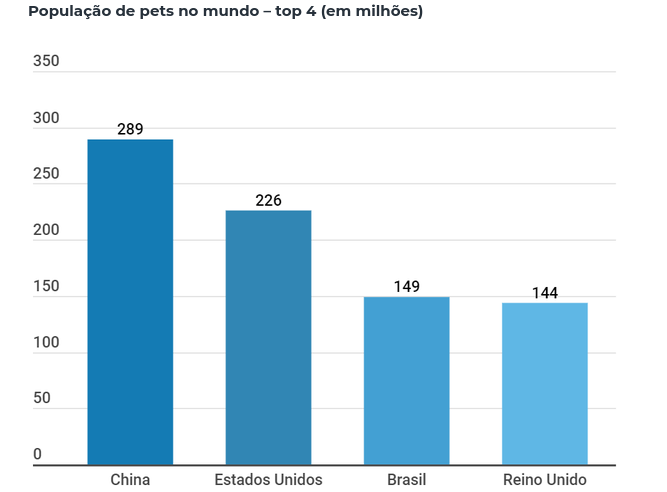
\includegraphics[
        width=0.5\linewidth,
        height=0.65\textheight,
        keepaspectratio
    ]{brasil_pets_mundo.png}
    %CORRIGIDO
    \fonte{\citeonline{panoramapetvet2023}.}
\end{figure}


%CORRIGIDO
Essa mudança de perfil social das famílias, em que o \textit{pet} passou a ser um membro de vital importância, tornou os tutores muito mais vigilantes e engajados com a transparência do cuidado do seu animal de estimação. Como consequência, todos os meios que se dedicam ao tratamento animal passaram a ser mais cautelosos com o bem-estar dos animais de estimação. A expansão da demanda por cuidados de saúde e bem-estar animal também se manifesta no ambiente de negócios. Levantamento do Sebrae, elaborado a partir de dados da Receita Federal, aponta que a abertura anual de pequenos negócios voltados ao mercado \textit{pet} passou de 12,7 mil, em 2023, para 15,5 mil, em 2025, o que corresponde a uma alta de 22\% no período \cite{sebrae2026}. No mesmo sentido, dados da Abinpet e do Instituto \textit{Pet} Brasil, divulgados por \citeonline{arbex2025}, indicam que o país ultrapassou a marca de 320 mil estabelecimentos do setor em 2024.

%CORRIGIDO
Ademais, notou-se uma mudança social expressiva no que tange à preocupação com a fauna urbana e doméstica. Essa maior consciência quanto à senciência e à valorização da vida animal reflete-se na criação e no endurecimento de arcabouços jurídicos, como a Lei Estadual nº 17.972/2024, de São Paulo, que reconhece cães e gatos como ``seres sencientes dotados de natureza biológica e emocional, passíveis de sofrimento'' \cite[art.~3º, IV]{saopaulo2024}, e a Lei Sansão (Lei nº 14.064/2020), que elevou as penas para crimes contra cães e gatos \cite{leisansao2020}, além do fortalecimento do terceiro setor (ONGs) para o acolhimento de animais vulneráveis. Esse movimento é reforçado pela atuação de organizações de proteção animal: segundo dados do Instituto \textit{Pet} Brasil, cerca de 4,8 milhões de cães e gatos vivem em situação de vulnerabilidade no país, dos quais mais de 201 mil estão sob a responsabilidade de ONGs \cite{oliveira2026}.

%CORRIGIDO
Paralelamente a essa expansão do mercado \textit{pet}, a transformação digital na saúde tem impulsionado a transição de registros físicos para sistemas de informação complexos \cite{pimazzoni2023}. No contexto da medicina veterinária, essa evolução não se limita apenas à substituição do papel, mas abrange a otimização de processos clínicos e a exigência de alta mobilidade profissional. A eficiência no diagnóstico e na conduta terapêutica está diretamente ligada à disponibilidade imediata do histórico do paciente. Contudo, essa premissa esbarra em um obstáculo técnico crítico em cenários de atendimento externo, visto que os profissionais dependem de dispositivos móveis e as aplicações atuais muitas vezes falham em suprir essa demanda operacional em locais com conexão instável ou ausente. A Figura~\ref{fig:cuidadoanimal} ilustra o cuidado clínico dispensado ao animal de estimação.

\begin{figure}[H] 
    \centering 
    %CORRIGIDO
    \caption{Ilustração do Cuidado Animal} 
    \label{fig:cuidadoanimal} 
    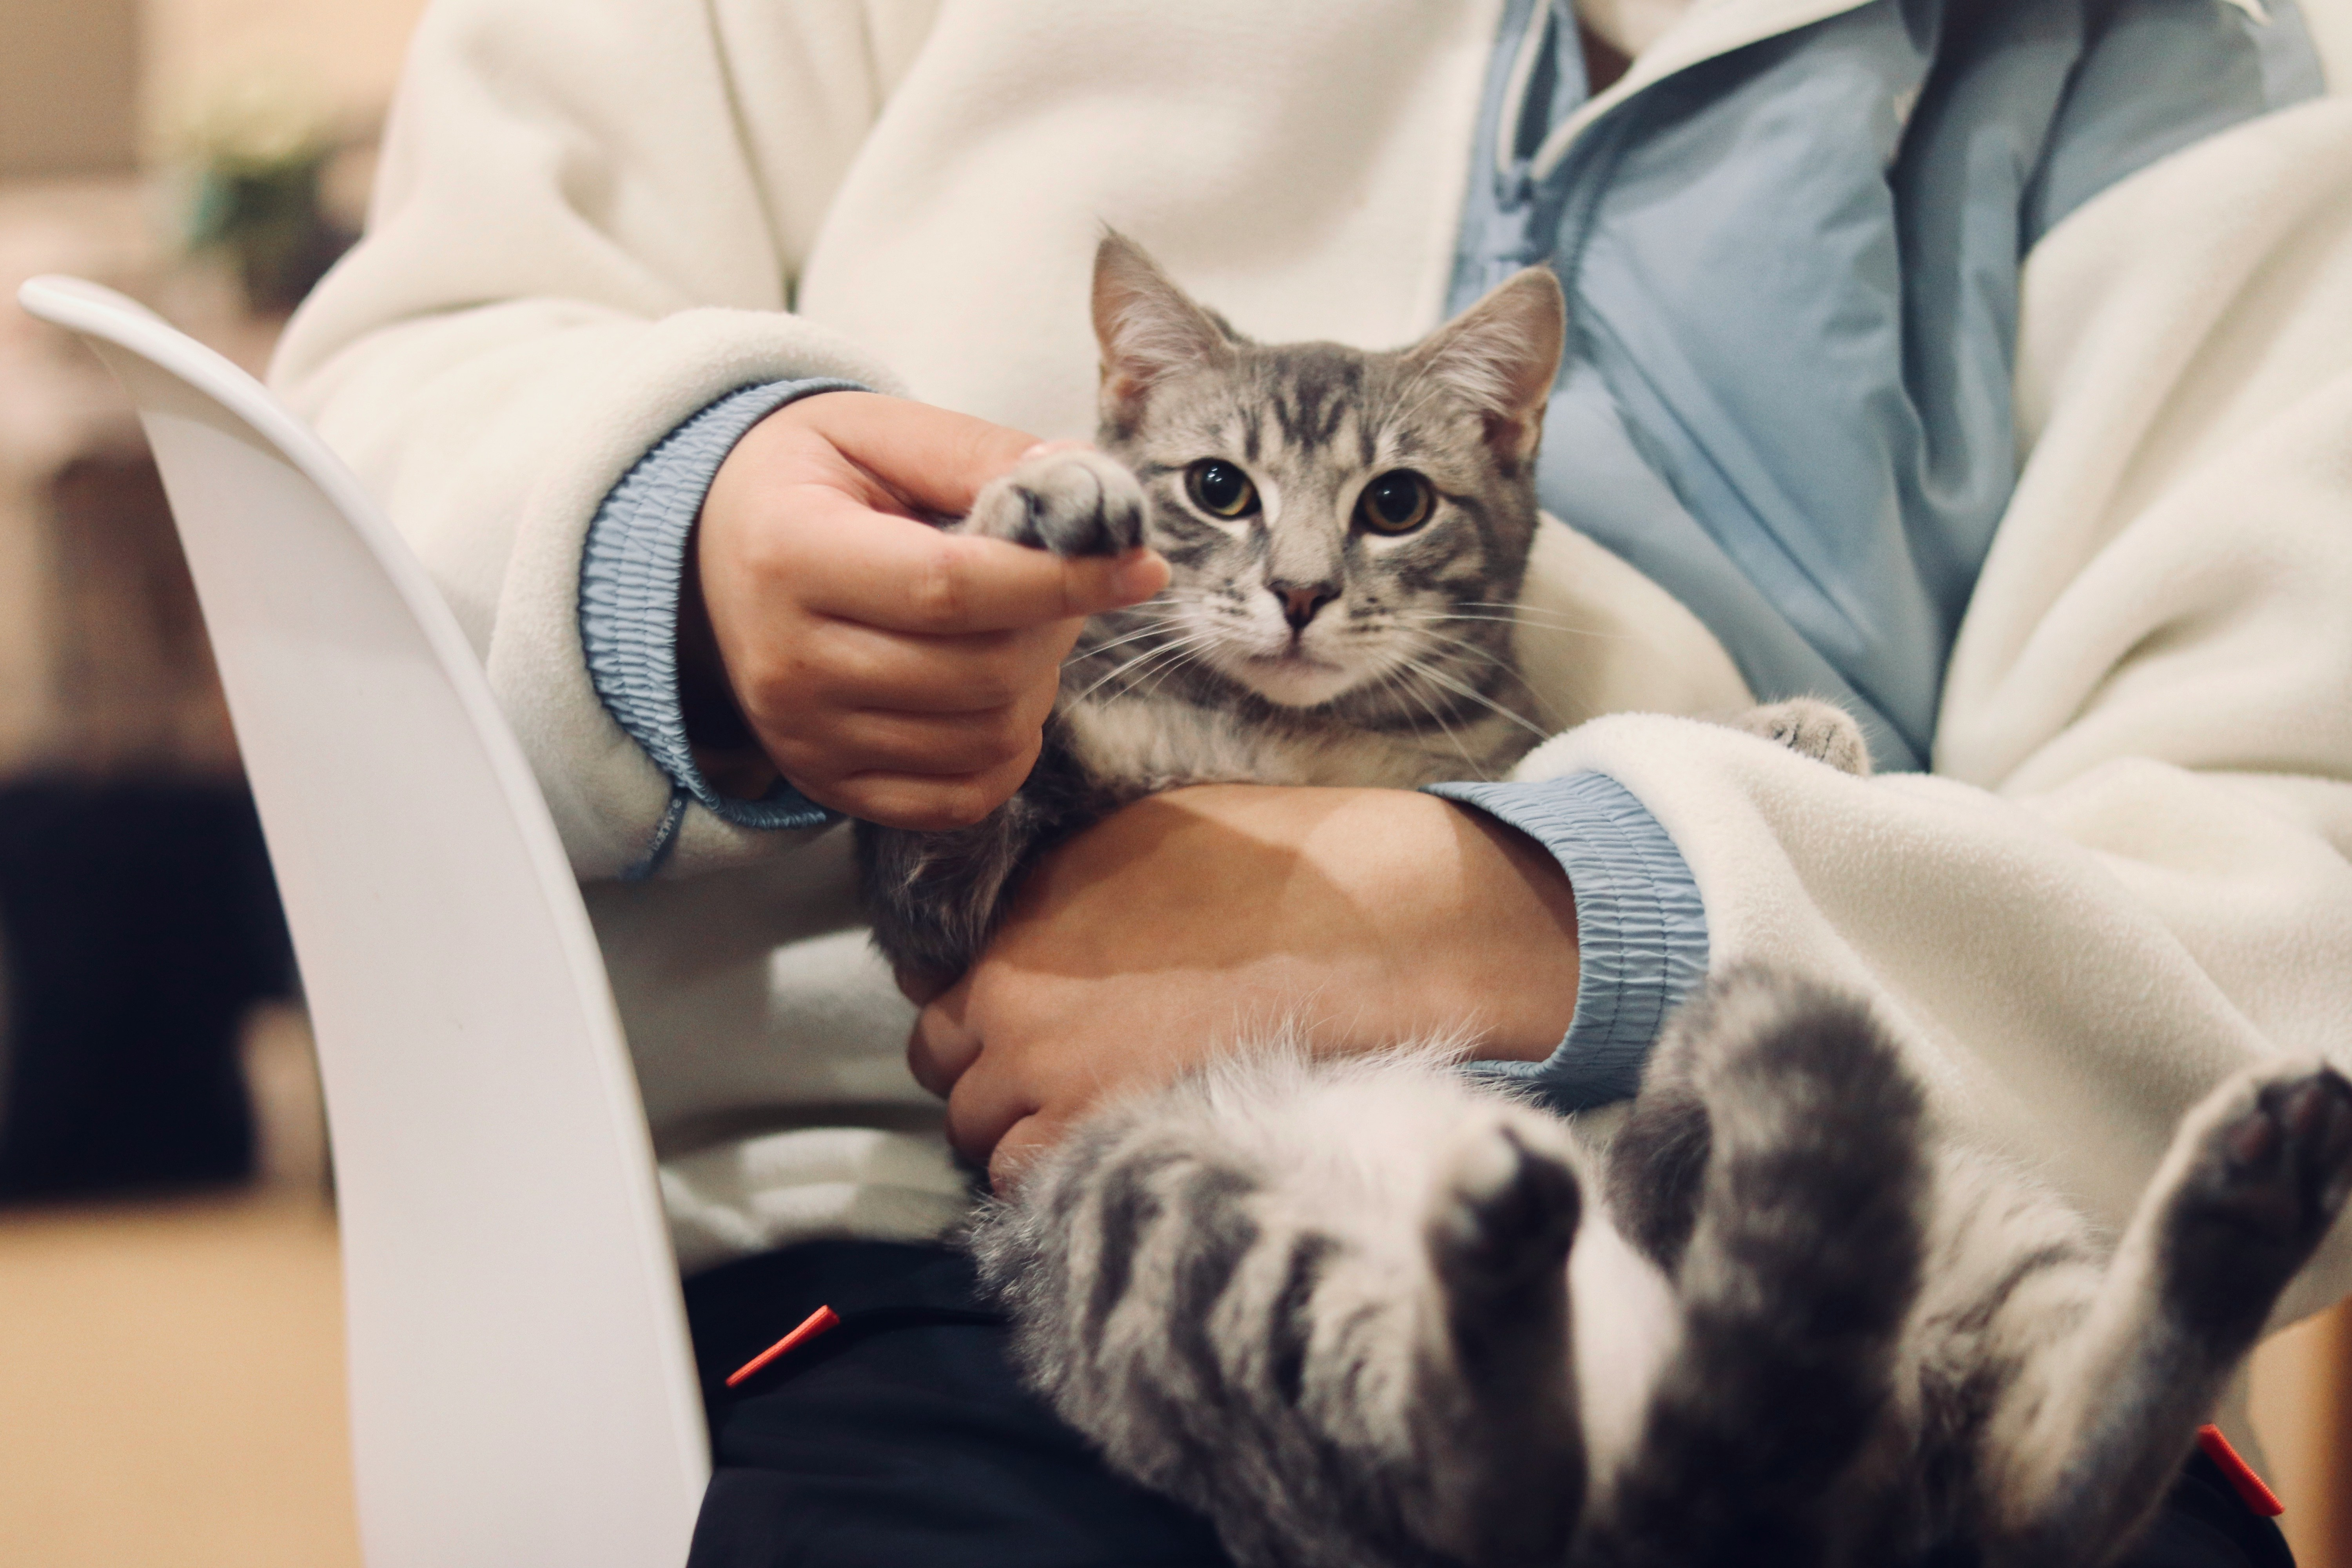
\includegraphics[
        width=0.5\linewidth,
        height=0.45\textheight,
        keepaspectratio
    ]{gato_vet.jpg}
    %CORRIGIDO
    \fonte{Werzk Luuuuuuu (\citeyear{werzk2020}).}
\end{figure}




\section{Estratégias de Persistência e o Paradigma Offline-First}
\label{sec:fundamentacao-teorica-a}
%CORRIGIDO
O conceito de \textit{offline-first} baseia-se na ideia de manipular dados quando não há conexão com a internet. Embora a maioria dos dados produzidos e compartilhados globalmente ocorra por meio da rede mundial de computadores, os sistemas \textit{offline-first} tratam a falta de conectividade não como um erro, mas como um estado previsível do sistema \cite{kleppmann2019}. Esse paradigma assume grande relevância na área de tecnologia da informação e no desenvolvimento de aplicações. Quando o foco principal de uma aplicação deixa de depender da presença de conexão com a internet, o paradigma atua como agente de persistência em sistemas desenvolvidos para operar de forma desconectada.

%CORRIGIDO
Diferentemente de sistemas que operam exclusivamente conectados e armazenam seus dados em servidores remotos, as aplicações que seguem esse paradigma utilizam o armazenamento local do dispositivo no qual são instaladas, seja um \textit{smartphone} ou um computador. Por meio da camada de cliente, com a qual o usuário interage, os dados são persistidos localmente, dessa forma, sempre que requisitados, são carregados dessa base local e exibidos ao usuário por meio de tecnologias como o \textit{WatermelonDB}, ferramenta integrada ao \textit{React Native} para a preservação de dados.

%CORRIGIDO
Embora esse modelo priorize os dados salvos localmente, a arquitetura ainda pode contar com um servidor remoto para possibilitar o funcionamento conectado. Portanto, na ausência de rede, os dados são manipulados de forma \textit{offline}, mas, quando o sinal retorna, a aplicação cliente sincroniza essas informações com o banco de dados principal, no servidor. Essa sincronização ocorre de forma assíncrona: quando a conexão é restabelecida, o sistema executa um protocolo de reconciliação para garantir que os dados inseridos localmente sejam integrados ao banco de dados principal no servidor de forma íntegra.

\section{Aspectos de Segurança e Proteção de Dados (LGPD)}
%CORRIGIDO
O crescimento constante das aplicações da área veterinária exige cuidado com a segurança do grande volume de dados gerados por seus usuários. Conforme estabelece a LGPD, Lei nº 13.709/2018 \cite{lgpd2018}, o tratamento de dados pessoais, inclusive nos meios digitais, realizado por pessoa natural ou por pessoa jurídica de direito público ou privado, deve proteger os direitos fundamentais de liberdade e de privacidade da pessoa natural. As decisões de segurança são pautadas na tríade CID (Confidencialidade, Integridade e Disponibilidade): a confidencialidade assegura que o acesso aos dados e sua divulgação ocorram somente de forma autorizada, protegendo-os, por exemplo, contra interceptações de terceiros a integridade protege os dados contra modificação ou destruição indevida e a disponibilidade garante o acesso oportuno e confiável aos dados e ao seu uso \cite[p.~2--3]{nist2017}.

%CORRIGIDO
Conforme é orientado, o tratamento dos dados coletados dos usuários será realizado somente nas hipóteses previstas no Artigo 7º da referida lei. Para a presente aplicação, consideram-se as seguintes hipóteses:

\begin{itemize}
     \renewcommand\labelitemi{-}
		%CORRIGIDO
		\item \textbf{Consentimento (Art. 7º, I):} trata da livre manifestação do usuário pela escolha do tratamento ou não tratamento dos seus dados pessoais.
		%CORRIGIDO
		\item \textbf{Cumprimento de Obrigação Legal ou Regulatória (Art. 7º, II):} justifica a coleta dos dados, quando requeridos por outras regulações, como resoluções do Conselho Federal de Medicina Veterinária (CFMV) ligadas à guarda e emissão de prontuários.
        %CORRIGIDO
        \item \textbf{Legítimo Interesse (Art. 7º, IX):} permite o tratamento dos dados quando necessário para atender aos interesses legítimos do controlador, exceto quando prevalecerem os direitos e liberdades fundamentais do titular.
	\end{itemize}

%CORRIGIDO
Além disso, vale destacar que o manuseio de dados pessoais relacionados a informações clínicas é integralmente regido pela LGPD. Em contrapartida, os dados referentes aos animais não se enquadram no escopo da Lei Geral de Proteção de Dados, portanto, qualquer informação inserida no sistema associada a um animal, como nome do \textit{pet}, espécie, raça, peso, temperatura, entre outros, é vinculada à pessoa natural que se caracteriza como seu tutor.
    \chapter{Trabalhos Relacionados}
\label{cap:trabalhos-relacionados}
%CORRIGIDO
Neste capítulo, são apresentados trabalhos que possuem similaridade com a proposta deste projeto, seja pelo domínio da aplicação, referindo-se ao setor veterinário, seja pela abordagem tecnológica, tratando-se de aplicações móveis ou de sincronização de dados.

\section{Prontuário Eletrônico Veterinário com Geolocalização (Pimazzoni, 2023)}
\label{sec:trabalho-relacionado-a}

%CORRIGIDO
O trabalho de \citeonline{pimazzoni2023} apresenta o desenvolvimento de um sistema de informações em saúde veterinária focado na integração de prontuários eletrônicos e geolocalização, com o objetivo de mapear áreas de maior incidência de zoonoses. A pesquisa destaca a necessidade de centralizar dados clínicos para melhorar a tomada de decisão do médico veterinário, além de estimular a atualização da base de dados com as infecções interespécie e seus respectivos vetores de transmissão, podendo tornar a prevenção e o tratamento futuro dessas doenças mais fáceis.

%CORRIGIDO
A aplicação VetWeb, desenvolvida a partir da pesquisa em questão, baseou-se no problema da escassez de dados públicos que tratem de doenças transmitidas entre animais e humanos, essas informações poderiam ser utilizadas posteriormente para pesquisas em saúde e disponibilizadas à população em geral, bem como no atraso gerado pela criação de prontuários manuais. O sistema possui telas voltadas para o cadastro de tutores, de pacientes e para a criação de prontuários clínicos, destinados à prescrição de exames, procedimentos e administração de vacinas. Além disso, cada paciente cadastrado na aplicação é devidamente localizado no mapa a partir do CEP fornecido em seu cadastro.

%CORRIGIDO
O sistema utiliza uma arquitetura cliente-servidor, além de estar disponível como aplicação \textit{mobile} e sistema \textit{web}, desenvolvido utilizando a linguagem PHP.




\section{Plataforma SimplesVet (Solução Comercial)}
\label{sec:trabalho-relacionado-b}
%CORRIGIDO
O SimplesVet \cite{simplesvet} é um dos principais \textit{softwares} de gestão veterinária no Brasil. Ele oferece módulos de prontuário, controle de estoque e financeiro, protocolos de vacina e planos pagos, operando majoritariamente no modelo \textit{Software as a Service} (SaaS). Essa aplicação auxilia no dia a dia dos veterinários, facilitando o trabalho em clínicas veterinárias, hospitais veterinários e \textit{pet shops}. É uma aplicação focada em empresas do ramo, pois além de fornecer as ferramentas para o uso do veterinário, ela também foca no controle financeiro da empresa que assina a plataforma, oferecendo telas para controle financeiro, como também estoque e serviços. 

%CORRIGIDO
Sobre a arquitetura do sistema, o SimplesVet foca em uma arquitetura baseada em nuvem, eliminando a necessidade de servidores locais. Além disso, os dados salvos no servidor da aplicação, vindos de diferentes pontos, são centralizados em uma única base de dados, como também a entrega desses dados em \textit{dashboards} profissionais, para medir o sucesso do SimplesVet no mercado, com o uso de métricas de desempenho.

%CORRIGIDO
Apesar de fornecer funcionalidades voltadas para o mercado veterinário, o SimplesVet opera no modelo SaaS, com os dados centralizados em nuvem, o que pressupõe a disponibilidade de conexão com a internet para o seu funcionamento. Dessa forma, a solução não é voltada ao público que atua em locais sem conectividade, como áreas isoladas de grandes cidades e regiões interioranas, cenário frequente no atendimento veterinário domiciliar. 



    

%CORRIGIDO
\section{Comparação entre os Trabalhos Relacionados}
\label{sec:trabalhos-relacionados-comparacao}
%CORRIGIDO
A Tabela~\ref{tab:trabalhos-relacionados} apresenta uma comparação entre os trabalhos relacionados e o RoadVet, considerando a adoção da arquitetura \textit{offline-first}, a presença de sincronização assíncrona e a portabilidade para dispositivos móveis.

%CORRIGIDO
\begin{table}[H]
    \centering
    \caption{Comparação entre os Trabalhos Relacionados}
    \label{tab:trabalhos-relacionados}
    \begin{tabular}{lccc}
        \toprule
        \textbf{Trabalho} & \textbf{Arquitetura \textit{offline-first}} & \textbf{Sincronização assíncrona} & \textbf{Portabilidade móvel} \\
        \midrule
        VetWeb     & Não & Não & Sim \\
        SimplesVet & Não & Não & Sim \\
        RoadVet    & Sim & Sim & Sim \\
        \bottomrule
    \end{tabular}
    \fonte{Elaboração própria.}
\end{table}



    \chapter{Metodologia}
\label{chap:metodologia}

%CARACTERIZTAR TODO O PROCESSO DE DESENVOLVIEMNTO DO TRABALHO, USANDO OS VERBOS NO FUTURO, DE FORMA QUE UMA PESSOA ENTENDA TODO O PROCESSOS DESTRINCHADO DE DESENVOLVIMENTO DO PROJETO.

A metodologia adotada para este trabalho fundamenta-se na pesquisa aplicada e no desenvolvimento experimental. O processo foi estruturado de forma a abranger a discussão com profissionais da área veterinária, o levantamento de requisitos, a definição da arquitetura do sistema, o desenvolvimento do projeto utilizando \textit{React Native} e \textit{Django Rest Framework} e, por fim, a realização de testes de sincronização em cenários de intermitência de rede.

%A PESQUISA É APENAS QUANTITATIVA! CORRIGIR ISSO
\section{Caracterização da Pesquisa}

O presente trabalho científico classifica-se como uma pesquisa aplicada. De acordo com Gil (2022), a pesquisa aplicada caracteriza-se pelo interesse prático, estando voltada para a aquisição de conhecimentos com vistas à aplicação direta e à solução de problemas específicos da realidade. No contexto desta pesquisa, o uso dessa abordagem é justificado pelo desenvolvimento de uma aplicação móvel com o objetivo de permitir que o antedimento em ambientes veterinário-domiciliares não seja interrompido pela perca de conexão com a internet.

Os objetivos desta pesquisa são caracterizados como exploratórios e descritivos. Apresenta caráter exploratório pois se aprofunda nos desafios de sincronização em cenários de baixa conectividade no atendimento domiciliar, como também se baseia em um problema pouco conhecido na sociedade. Adicionalmente, manifesta-se como descritiva ao detalhar o comportamento e a eficiência das tecnologias utilizadas, com foco no \textit{framework} \textit{Django Rest Framework} e na biblioteca \textit{React Native}, demonstrando como chegar ao resultado final, desde o levantamento de requisitos até a aplicação final.

A abordagem do seguinte trabalho se caracteriza como quantitativa, se revela dessa forma quando se preocupa com a sincronização dos dados e com a persistência dos deles, tanto na camada de suporte como na camada de cliente.
%A ABORDAGEM É NA VERDADE QUANTITATIVA

A metodologia adotada nesta pesquisa fundamenta-se no método da engenharia, alinhado à \textit{Design Science Research} (DSR), visto que o trabalho busca solucionar um problema prático vivenciado por médicos veterinários que atuam em domicílio. O percurso metodológico seguiu o ciclo heurístico composto pelas etapas de: identificação das principais necessidades dos veterinários domiciliares, mapeamento dos requisitos de persistência local, projeto da arquitetura \textit{offline-first}, implementação do protótipo funcional e avaliação da eficácia do sistema sob condições simuladas de falta de conectividade.
    
\pagebreak

Quanto aos procedimentos técnicos, o trabalho baseia-se no desenvolvimento experimental. Essa vertente envolve a execução de testes manuais em cenários simulados de ausência e restabelecimento de conexão, permitindo validar empiricamente a eficácia dos mecanismos de sincronização e persistência dos dados manipulados.

\section{Discussões com Profissionais da área Veterinária}
Para o desenvolvimento deste trabalho, o primeiro passo consistiu em contatar profissionais da área veterinária, preferencialmente atuantes de forma autônoma, com o objetivo de iniciar conversas a respeito de sua rotina diária e de identificar as principais dificuldades encontradas no exercício da profissão. Essas interações foram conduzidas de maneira aberta e colaborativa, permitindo que os profissionais relatassem as nuances percebidas ao longo de sua trajetória e auxiliassem na definição dos pontos prioritários a serem considerados no desenvolvimento do aplicativo. Todas as propostas consideradas viáveis e aplicáveis ao escopo do projeto foram devidamente registradas e utilizadas posteriormente para embasar o levantamento de requisitos.

\section{Levantamento de Requisitos}
%TRAZER UMA LISTA DOS REQUISITOS DO NOTION
Após a primeira etapa de reconhecimento dos principais problemas que assolam os veterinários domiciliares, foram definidos os requisitos da aplicação, divididos em funcionais e não funcionais, essas definições foram primordiais para promover uma maior organização de prioridades no desenvolvimento do aplicativo. Requisitos funcionais são as funcionalidades indispensáveis da aplicação, aquelas que não podem deixar de ser implementadas, pois são básicas para a resolução do problema que é proposto a ser resolvido pelo sistema, já os requisitos não funcionais se caracterizam-se como os atributos de qualidade, restrições e critérios técnicos que moldam a forma como o sistema opera, abrangendo aspectos de segurança, desempenho e arquitetura.

Para anotar os requisitos do presente projeto, foi utilizada a ferramente\textit{ Notion}, que funciona como um organizador de ideias e anotações digital, na plataforma citada, foi definido um módulo que classificou os requisitos como funcionais e não funcionais, como também classificou sua prioridade de aplicação, divididos em média, baixa e alta prioridade, influenciando diretamente nas decisões finais do aplicativo conforme era posto em prática a digitação do código.

A fim de ilustrar a estrutura adotada, estão representados abaixo alguns requisitos que se detacam como de maior importância para o sistema. A lista completa de todos os requisitos encontra-se disposto no Apêndice ~\ref{ap:requisitos} deste trabalho.

%DEIXAR 5 REQUISITOS FUNCIONAIS E NÃO FUNCIONAIS E COLOCAR O RESTO PARA O APÊNDICE
\subsection{Requisitos Funcionais (RF) (Amostra)}

\begin{itemize}
    \item \textbf{RF01 -- Cadastrar veterinários:} A aplicação deve permitir o cadastro de veterinários mediante identificador, nome, e-mail e senha, com CRMV e telefone opcionais.

    \item \textbf{RF10 -- Gerenciar Prontuários:} A API deve permitir cadastrar, consultar, atualizar e excluir logicamente prontuários vinculados a animais e ao veterinário responsável.

    \item \textbf{RF20 -- Sincronização Assíncrona:} O sistema deve detectar automaticamente o restabelecimento da conexão Wi-Fi ou Dados Móveis e realizar o upload dos dados pendentes sem interromper a navegação do usuário.

    \item \textbf{RF24 -- Operar sem conexão:} A aplicação deve permitir consultar e manter tutores, animais e prontuários localmente sem conexão, sincronizando posteriormente.

\end{itemize}

\subsection{Requisitos Não Funcionais (RNF) (Amostra)}

\begin{itemize}
    \item \textbf{RNF01 -- Autenticação das operações protegidas:} A API deve exigir autenticação JWT para sincronização e envio de arquivos.
    
    \item \textbf{RNF04 -- Isolamento dos dados entre veterinários:} A API deve restringir estritamente as operações aos dados associados ao veterinário autenticado.
    
    \item \textbf{RNF05 -- Atomicidade do recebimento de alterações:} As alterações recebidas em uma requisição de sincronização devem ser processadas em uma única transação de banco de dados, sendo revertidas caso ocorra uma falha que interrompa a operação.
    
    \item \textbf{RNF10 -- Persistência local:} O aplicativo deve preservar registros entre execuções e permitir acesso offline.
    
\end{itemize}

\section{Definição da Arquitetura de Sistema e Desenvolvimento da Aplicação}
%FALAR DE MANEIRA GERAL
Após o estudo dos diversos tipos de aplicações móveis, foram definidas as arquiteturas para as diferentes camadas do sistema. Inicialmente, estruturou-se a arquitetura de banco de dados, que reúne o modelo de cada entidade envolvida na lógica de negócio, especificando os tipos de campos, como chaves primárias e tipos primitivos de dados e as respectivas relações entre as tabelas. Em seguida, definiu-se a arquitetura de front-end, responsável pela construção da interface do usuário e da persistência de dados local. Por fim, estruturou-se a camada do servidor, que centraliza a lógica de negócio e o gerenciamento das requisições globais.

\section{Procedimentos de Validação e Testes}
Para validar o funcionamento da aplicação, foi projeto um ambiente de testes controlado, que buscou se aproximar de situações reais vividas pelos profissionais da área veterinária domiciliar. Durante a fase de testes, as camadas de cliente e de suporte foram testadas individualmente e em conjunto, em situações com e sem presença de internet.

Quanto ao procedimento de teste, a aplicação foi executada em ambiente emulado, inicializando-se a API e a interface móvel (\textit{front-end}) de forma simultânea. Em seguida, foram efetuados registros de dados fictícios — primeiramente sob conectividade plena e, em seguida, com a interrupção intencional da rede —, a fim de validar a persistência local no modo \textit{offline}. Por fim, a conexão foi restabelecida para verificar a correta sincronização assíncrona dos dados com o servidor central.
    \chapter{Roadvet}
\label{cap:roadvet}
Este capítulo apresenta a contribuição principal deste trabalho, a aplicação RoadVet.

\section{Definição da Arquitetura do Sistema}

A arquitetura do sistema foi projetada segundo o modelo Cliente-Servidor, utilizando o padrão de \textit{APIs REST.} Essa abordagem justifica-se pelo fato de possibilitar o desacoplamento entre interface do usuário e regras de negócio, que no contexto do ambiente veterinário domiciliar é fundamental. Dessa maneira, o modelo Cliente-Servidor fornece uma independência ao cliente, de forma que os dados são processados localmente sem a necessidade da conexão com a internet. Assim quando a comunicação é reestabelecida com o servidor, a \textit{API REST} garante a comunicação entre ambos e salva os dados pendentes no banco de dados, conforme ilustrado na Figura~\ref{fig:arquitetura}.

%MODELAR A ARQUITETURA DO SISTEMA

\begin{figure}[H] 
    \centering 
    \caption{Diagrama de Arquitetura do Sistema} 
    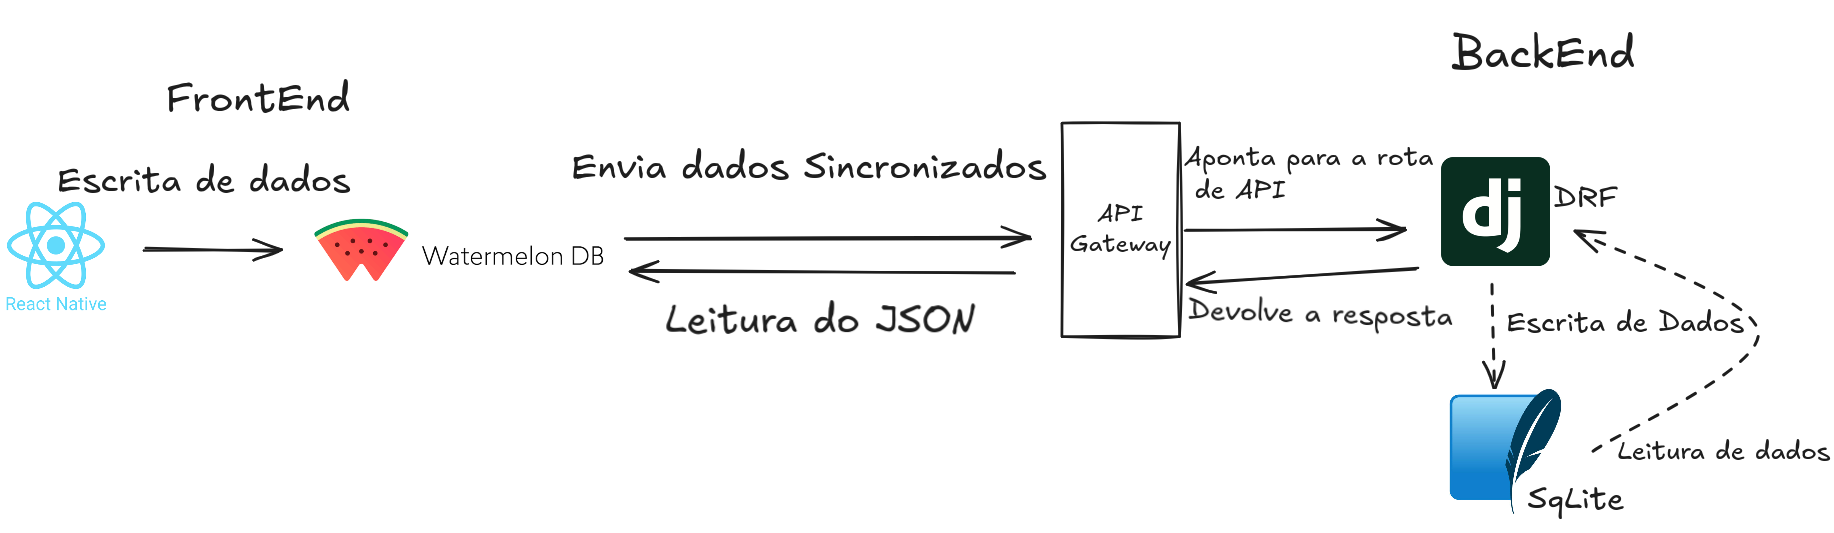
\includegraphics[width=\linewidth]{ArquiteturaSistema.png} 
    \label{fig:arquitetura} 
    \vskip 3pt
    \fonte{Elaboração própria}
\end{figure}


\section{Visão Geral}
% <<< REVISAR O TEXTO, POIS CITA QUE O APP TAMBÉM ATENDE PESSOAS SEM CRMV >>>
%EXPLICAR PARA QUEM É A APLICAÇÃO, MOSTRAR O FLUXO DETALHADO
%FAZER RELAÇÃO DAS TELAS COM OS REQUISITOS CITADOS
%NÃO DEIXAR IMAGENS UMA ABAIXO DA OUTRA SEM TEXTO
O RoadVet foi desde o princípio pensado com cuidado para atender os profissionais veterinários que se deslocam para atendimentos em regiões onde a rede mundial de computadores não funciona de forma devida, portanto a presente aplicação primordialmente atende à esses trabalhadores, de qualquer nível e que zelam pela saúde animal de forma autônoma, não impossibilitando que seja usado por profissionais de clínicas e estudantes em ambientes que possuem forte conexão com a internet, já que o aplicativo também opera normalmente com a presença de conexão, possibilitando o cadastro de pets, tutores e a criação de prontuários clínicos. No que tange a portabilidade do aplicativo, é importante destacar que ele foi pensado e desenvolvido para funciona especificamente em plataformas mobile, portanto não há a possibilidade de executá-lo em computadores de mesa ou notebooks.

\subsection{Fluxo Principal do Sistema}
Em relação ao fluxo do sistema e o primeiro contato do usuário com o RoadVet, o usuário é apresentado à tela de boas-vindas que consiste em dois botões: o primeiro destinado a cadastrar o novo usuário, redirecionando para uma tela de formulário de cadastro, o segundo para os usuários já cadastrados na plataforma, que redireciona para a tela de login. Esta tela é apresentada na Figura~\ref{fig:boasvindas}:

\begin{figure}[H] 
    \centering 
    \caption{Tela de Boas-Vindas do aplicativo} 
    \label{fig:boasvindas} 
    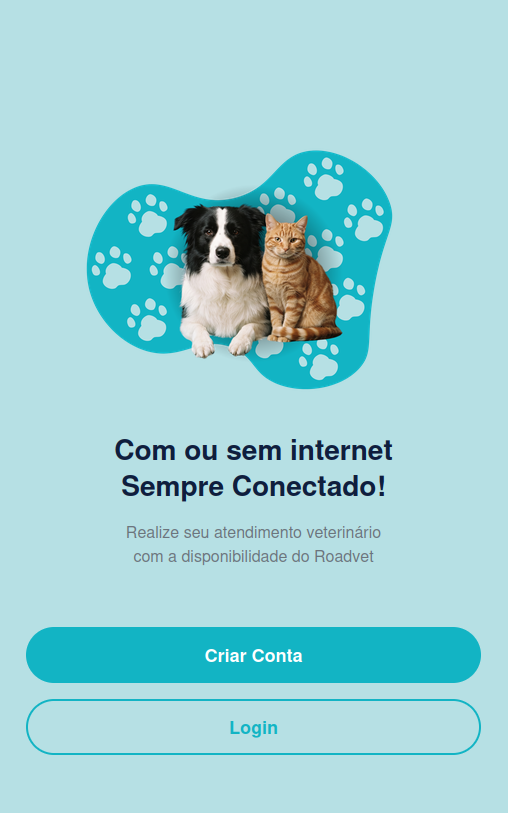
\includegraphics[
        width=0.5\linewidth,
        height=0.65\textheight,
        keepaspectratio
    ]{telaDeBoasVindasApp.png}
    \fonte{Elaboração própria.}
\end{figure}

Prosseguindo com esse fluxo, o usuário recém chegado irá clicar no botão de "Criar conta" e será redirecionado para o formulário aonde serão coletados seus dados pessoais, são eles nome completo, crmv, que é a licença que permite a prática formalizada da profissão do veterinário, email pessoal, telefone com DDD e senha, após isso o usuário será salvo no banco de dados do servidor. Segue a representação na figura ~\ref{fig:cadastro}:

\begin{figure}[H] 
    \centering 
    \caption{Tela de Cadastro do Aplicativo} 
    \label{fig:cadastro} 
    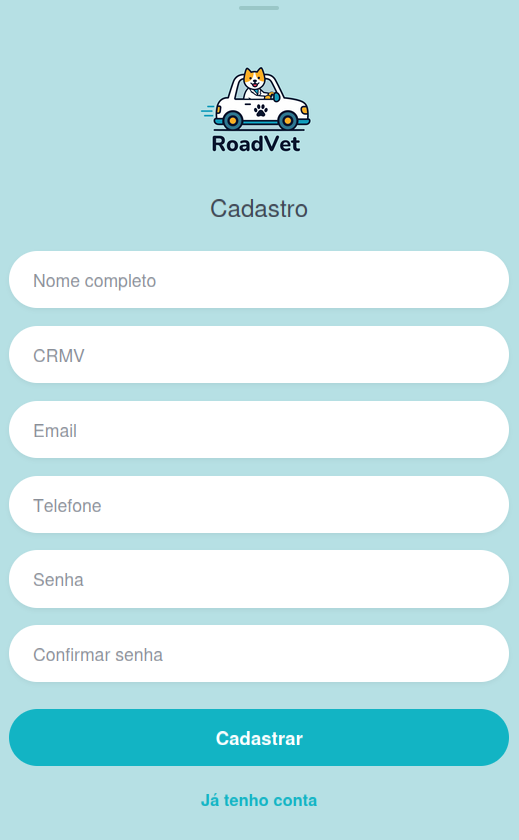
\includegraphics[width=0.5\linewidth]{teladDeCadastroApp.png}
    \fonte{Elaboração própria.}
    \vskip 3pt 
    \noindent{\small} 
\end{figure}

No caso de já existir um cadastro para o usuário, basta clicar no botão "Login", na tela de boas vindas, demonstrado na figura ~\ref{fig:boasvindas} e informar o email e senha para seguir os próximos passos, a tela de login está representada na figura ~\ref{fig:login}:

\begin{figure}[H] 
    \centering 
    \caption{Tela de Login do Aplicativo} 
    \label{fig:login} 
    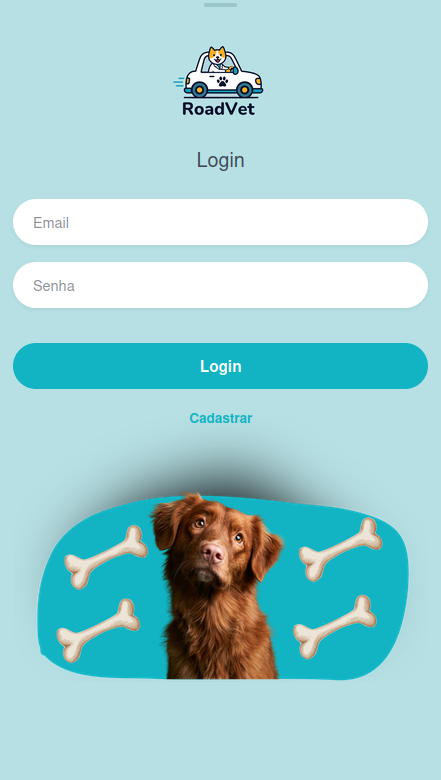
\includegraphics[width=0.5\linewidth]{telaDeLoginApp.png}
    \fonte{Elaboração própria.}
    \vskip 3pt 
    \noindent{\small} 
\end{figure}

Após a criação da conta, o veterinário será automaticamente direcionado para a tela principal do sistema, aonde o usuário é recebido com boas vindas no canto superior da tela, como também apresenta os ícones que descrevem que ele está com a conexão funcionando e o ícone de sair da conta, nessa ordem, os outros ícones redirecionam para a criação de um nova consulta, novo tutor, novo pet, lista de pacientes(pets), lista de tutores e o histórico de atendinentos, também nessa ordem. Logo abaixo está o painel de acompanhamento das últimas consultas feitas por ele, além da mensagem que reforça a sincronização com a internet. 

Nessa tela o usuário se depara com ícones na barra inferior da tela, o primeiro leva a tela atual, o segundo trata de todas as ações relativas aos pets, como criação, listagem e atualização, o terceiro trata das funcionalidades da entidade de tutores e o último é o ícone que leva à tela de prontuários e é nele que o usuário vai se redirecionar de acordo com o fluxo atual. Logo ao entrar nessa tela é possível pesquisar os prontuários existentes por nome, data e descrição, além da pesquisa é possível ordenar por cadastro mais recente, tutor ou pet em ordem alfabética e há a opção de filtrar canino, felino, com prescrição e sem prescrição. Todas as funcionalidades referentes aos prontuários estão disponíveis nessa tela, é possível criar um novo prontuário, ver a listagem deles, com nome do pet, data de criação e se é um cachorro ou gato, como também possui o ícone que mostrar se há ou não sincronização com o servidor. Segue uma representação fiel dessa tela na figura ~\ref{fig:painel}:

\begin{figure}[H] 
    \centering 
    \caption{Painel Principal do Aplicativo} 
    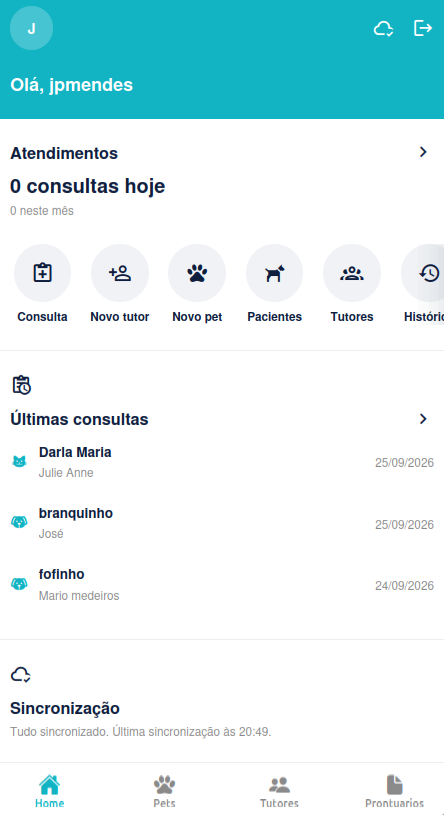
\includegraphics[width=0.5\linewidth]{painelPrincipalApp.png} 
    \fonte{Elaboração própria.}
    \label{fig:painel} 
    \vskip 3pt 
    \noindent{\small} 
\end{figure}

O próximo passo é clicar no quarto ícone  chamado "Prontuários", na parte inferior direita da tela, é nessa tela que acontece a orquestração dos prontuários, à primeira vista já é mostrada a listagem dos prontuários que já foram criados com o nome dos pets e data de criação, após essa ação o usuário é finalmente redirecionado para a tela de prontuários clínicos do aplicativo, representada na figura  ~\ref{fig:prontuarios}:

\begin{figure}[H] 
    \centering 
    \caption{Tela de Prontuários do Aplicativo} 
    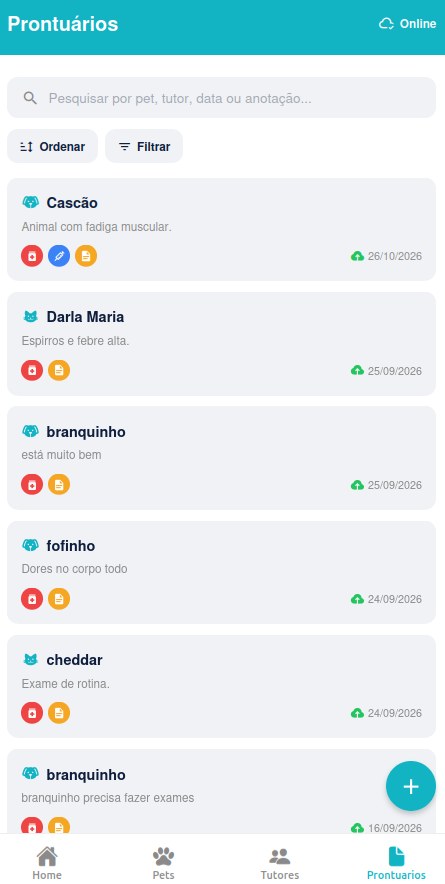
\includegraphics[width=0.5\linewidth]{telaDeProntuariosApp.png} 
    \fonte{Elaboração própria.}
    \label{fig:prontuarios} 
    \vskip 3pt 
    \noindent{\small} 
\end{figure}

Seguindo o fluxo que está sendo representado, a próxima ação é clicar no ícone de "+" no canto inferior direito da tela, depois disso o veterinário é finalmente levado a tela de criação do prontuário clínico, aonde são mostrados os pets que já estão cadastrados, com o nome de seu tutor ao lado. Além disso a tela conta com uma barra de pesquisas no canto superior, que permite filtrar os pets por nome, raça ou tutor relacionado. Abaixo dessa barra está representado o botão "+ Novo pet", responsável pela criação de um novo pet, caso seja o primeiro prontuário criado para ele, caso o pet já exista basta selecioná-lo na lista. A tela está representada na figura ~\ref{fig:criacaoprontuariolista}:

%\clearpage

\begin{figure}[H] 
    \centering 
    \caption{Tela de Criação de Prontuário} 
    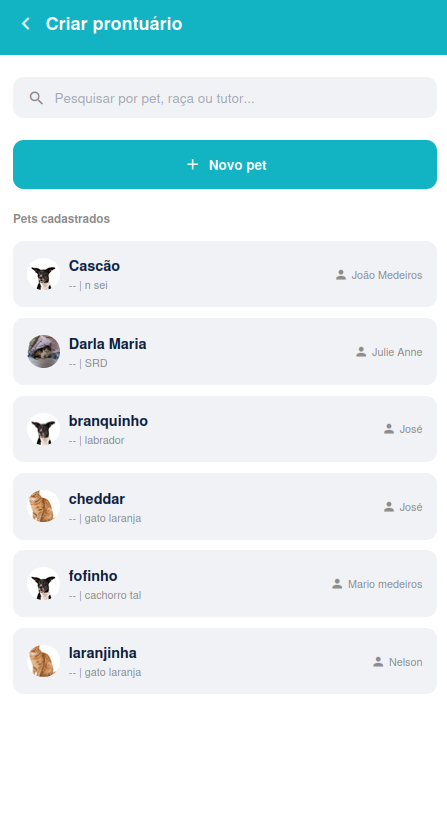
\includegraphics[width=0.5\linewidth]{TelaProntuarioCriacaoApp.png} 
    \fonte{Elaboração própria.}
    \label{fig:criacaoprontuariolista} 
    \vskip 3pt 
    \noindent{\small} 
\end{figure}

Após escolher uma entre as duas formas possíveis de criar o pet para o prontuário, o próximo passo é preencher o formulário de criação desse prontuário, devem ser fornecidos os seguintes dados em ordem: peso do animal em quilogramas, temperatura do animal em graus celsius, frequência cardíaca do animal, um texto referente a anamnese feita pelo veterinário, um texto para relatar o exame físico realizado, um texto com a prescrição após finalizar o exame e outros dados que serão informados na captura de tela seguinte, o que foi descrito está representado na figura ~\ref{fig:formularioprontuario1}:

%\clearpage

\begin{figure}[H] 
    \centering 
    \caption{Tela de Criação de Prontuário 1} 
    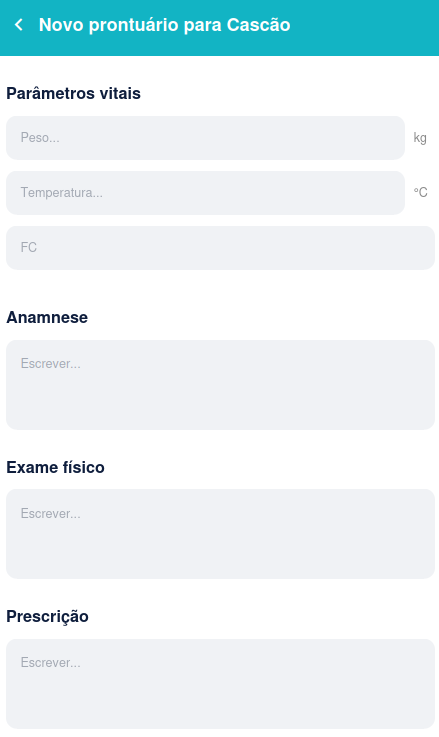
\includegraphics[width=0.5\linewidth]{TelaFormulario1.png} 
    \fonte{Elaboração própria.}
    \label{fig:formularioprontuario1} 
    \vskip 3pt 
    \noindent{\small} 
\end{figure}

Ainda no preenchimento do formulário, é preciso também inserir os dados de texto referentes a vacinas, solicitação de exames com anexo de PDF ou imagem e um texto contendo os resultados finais desse atendimento, também com anexo de PDF ou imagem e por fim salvar esse prontuário ou cancelar caso seja percebido algum erro. A tela está representada na figura ~\ref{fig:formularioprontuario2}:

%\clearpage

\begin{figure}[H] 
    \centering 
    \caption{Tela de Criação de Prontuário 2} 
    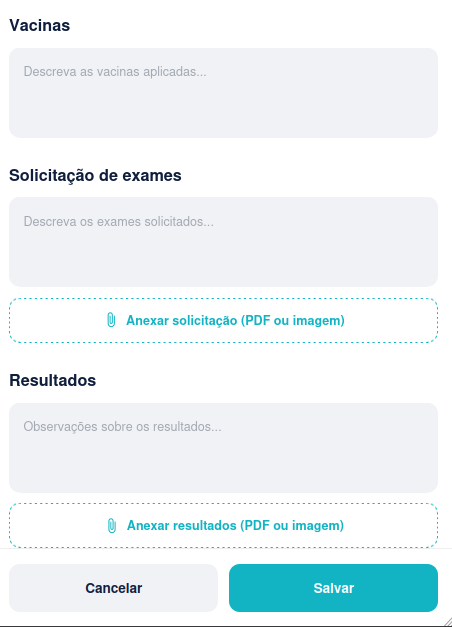
\includegraphics[width=0.5\linewidth]{FormularioProntuario2.png} 
    \fonte{Elaboração própria.}
    \label{fig:formularioprontuario2} 
    \vskip 3pt 
    \noindent{\small} 
\end{figure}

No caso do pet ainda não estar cadastrado no sistema, será necessário optar pela opção "Novo pet", logo abaixo da barra de pesquisa na tela, conforme foi apresentado na figura ~\ref{fig:criacaoprontuariolista}, serão preenchidas as informações para criar um novo pet, gato ou cachorro, deve-se fornecer imagem, o tutor responsável, caso já existam tutores cadastrados, nome, data de nascimento, peso em quilogramas, espécie e raça, depois basta clicar em "salvar" para cadastrar o animal ou "cancelar" caso haja algum erro. Segue na figura ~\ref{fig:criacaopet}, o que foi descrito agora.

%\clearpage

\begin{figure}[H] 
    \centering 
    \caption{Tela de Criação de Pet} 
    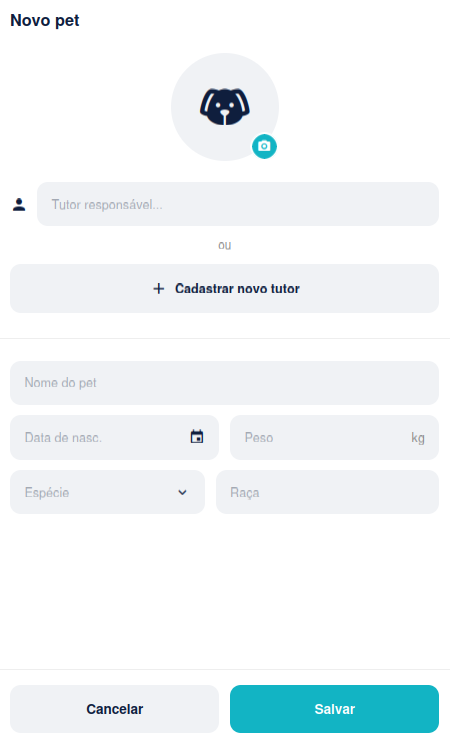
\includegraphics[width=0.5\linewidth]{NovoPetProntuario.png} 
    \fonte{Elaboração própria.}
    \label{fig:criacaopet} 
    \vskip 3pt 
    \noindent{\small} 
\end{figure}

No caso da não existência do tutor relacionado ao pet desejado, é possível clicar no botão "Cadastrar novo tutor", logo abaixo da opção "Tutor responsável", como mostrado na figura ~\ref{fig:criacaopet}, o usuário será redirecionado para a tela de cadastro do tutor, aonde serão fornecidos os dados de imagem, nome completo, cpf, data de nascimento, email, CEP, endereço, número, bairro, complemento, cidade, unidade federativa e dois telefones para contato. Isso é representado na figura ~\ref{fig:criacaotutor}

\clearpage

\begin{figure}[!htbp] 
    \centering 
    \caption{Tela de Criação do Tutor} 
    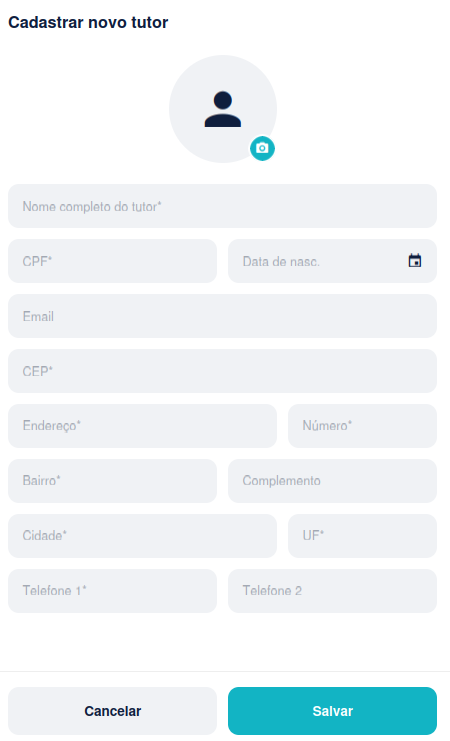
\includegraphics[width=0.5\linewidth]{CadastroTutorApp.png} 
    \fonte{Elaboração própria.}
    \label{fig:criacaotutor} 
    \vskip 3pt 
    \noindent{\small} 
\end{figure}

Se o passo a passo for seguido corretamente como descrito a cima, no final o usuário terá um prontuário profissional em seu aplicativo, totalmente funcional e aberto para edições e exclusão, em modo online e offline.

\section{Desenvolvimento do Aplicativo}
O desenvolvimento da aplicação foi executado fundamentando-se nos princípios e ensinamentos da Engenharia de Software, visando à construção de uma solução técnica plenamente funcional, modular e escalável. O sistema foi estruturado de forma desacoplada, dividindo-se entre a camada do cliente (\textit{front-end} móvel) e a camada de suporte (\textit{back-end}), permitindo a distribuição isolada das responsabilidades e a aplicação rigorosa das regras de negócio.

Como Ambiente de Desenvolvimento Integrado (\textit{Integrated Development Environment}, IDE) para ambas as vertentes do ecossistema, utilizou-se o \textit{Visual Studio Code} (\textit{VS Code}). O gerenciamento de configuração e o versionamento do código-fonte foram realizados por meio da ferramenta \textit{Git}, com o mapeamento sistemático dos incrementos em um repositório remoto hospedado na plataforma \textit{GitHub}. Essa abordagem garantiu a redundância do código-fonte entre a estação local de trabalho e o servidor remoto, servindo como um mecanismo de contingência para a recuperação de dados em caso de falhas de \textit{hardware}. Além disso houve a escolha do WatermelonDB como mecanismo de persistência local, garantindo assim o funcionamento do aplicativo somente na camada do cliente, em caso de perda de conexão. Reconhece-se que, para um ambiente de produção real e escalável no setor de saúde, a tecnologia chave-valor apresenta restrições de performance e segurança se comparada a bancos de dados relacionais locais como \textit{SQLite }ou documentais como \textit{Realm}.

No escopo da camada do cliente, a biblioteca \textit{React Native} foi adotada para o desenvolvimento da interface e da camada de apresentação do usuário. Nessa estrutura, implementou-se a lógica de persistência local utilizando a biblioteca \textit{AsyncStorage}, o que viabilizou a execução de operações fundamentais de criação, consulta, atualização e exclusão (\textit{Create, Read, Update and Delete}, CRUD) de prontuários clínicos diretamente no dispositivo móvel, mitigando os impactos decorrentes da falta de conectividade em campo.

Para a camada de suporte, utilizou-se o \textit{Django Rest Framework} (DRF) para a construção de uma API REST baseada na linguagem de programação \textit{Python}, enquanto o sistema gerenciador de banco de dados relacional \textit{SQLite} foi definido para a persistência e o armazenamento estruturado das informações. A lógica de negócio desenvolvida na retaguarda concentrou-se no gerenciamento da sincronização dos dados provenientes do cliente móvel. Desse modo, estabeleceu-se que, na presença de conexão ativa, as requisições são processadas e persistidas de forma imediata no banco de dados principal; em cenários de intermitência, o fluxo de dados aguarda a validação e as diretivas de sincronização disparadas pela camada superior da aplicação, mantendo a integridade das operações de criação, visualização, atualização e deleção.

\section{Estratégia de Persistência e Sincronização}
As estratégias utilizadas para persistir e sincronizar os dados em ambas as camadas projetadas no sistema foram estruturadas seguindo o conceito de arquitetura \textit{offline-first}. Essa abordagem garante que a aplicação móvel permaneça plenamente operacional para o médico veterinário mesmo em locais sem cobertura de rede, postergando a comunicação com o servidor para o momento em que a conectividade for restabelecida.

%REVISAR ESSE PARÁGRAFO
Na camada do cliente \textit{(front-end)}, o mecanismo de persistência local fundamenta-se na utilização da biblioteca \textit{WatermelonDB}. Por se tratar de um banco de dados reativo e local estruturado sobre o SQLite, a ferramenta permite gerenciar os dados relacionais dos prontuários clínicos diretamente no dispositivo de forma assíncrona. Para viabilizar o controle do fluxo de dados, cada registro manipulado localmente incorpora metadados de controle, especificamente uma marca temporal \textit{(timestamp)} da última modificação e uma flag indicadora de status de sincronização mapeada entre os estados pendente e sincronizado.

O processo de sincronização foi projetado a partir de uma estrutura de fila de eventos, cujo comportamento operacional é ditado pela detecção dinâmica do estado da rede, conforme descrito a seguir:

\begin{itemize}
    \item \textbf{Fluxo em Modo Offline:} Caso o dispositivo detecte a ausência de conexão à internet ou as requisições HTTP retornem falha por indisponibilidade de rede, as operações de CRUD são desviadas e executadas estritamente no \textit{WatermelonDB}. O registro correspondente é marcado com o \textit{status} de pendente e a operação é empilhada na fila local de sincronização.
    %REVER COMO FUNCIONA AGORA, CRIEI UMA ROTA ASYNC PARA A SINCRONIZAÇÃO
    \item \textbf{Fluxo em Modo Online e Reconexão:} Ao identificar o restabelecimento de uma conexão ativa e estável, a aplicação móvel inicia o esvaziamento da fila de maneira assíncrona. As operações pendentes são transmitidas sequencialmente à camada de suporte por meio de requisições HTTP utilizando os verbos adequados (\textit{POST} para criações, \textit{PUT} ou \textit{PATCH} para atualizações e \textit{DELETE} para exclusões), direcionadas aos respectivos \textit{endpoints} da API.
\end{itemize}

\begin{figure}[H] 
    \centering 
    \caption{Demonstração de Sincronização Bem-Sucedida no App} 
    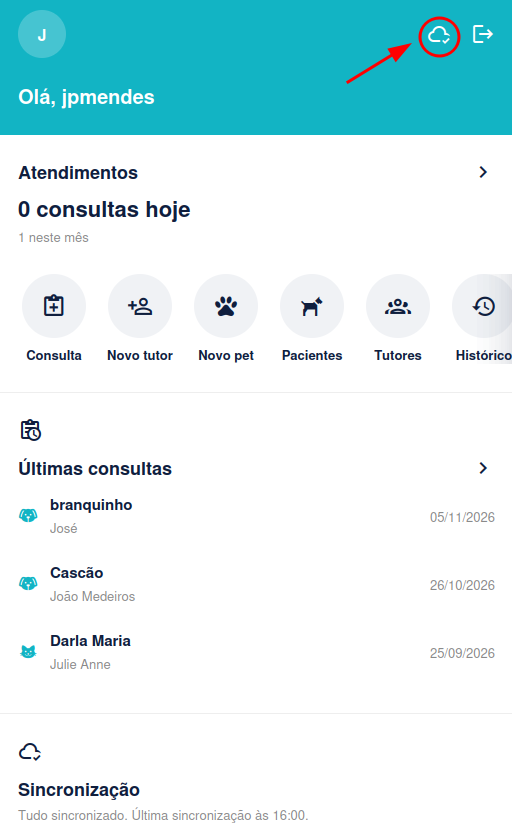
\includegraphics[width=0.5\linewidth]{sincronizacaoCap.png} 
    \fonte{Elaboração própria.}
    \label{fig:sincronizacaoCap} 
    \vskip 3pt 
    \noindent{\small} 
\end{figure}

Na camada de suporte (\textit{back-end}), o \textit{Django Rest Framework} (DRF) atua como o receptor e validador do lote de dados transmitidos pelo cliente móvel. Ao receber as requisições de sincronização, as rotas da API acionam as regras de negócio e os serializadores (\textit{serializers}) para garantir a integridade e consistência das informações antes de persisti-las de forma definitiva no banco de dados relacional \textit{SQLite}.

Para a resolução de potenciais conflitos de concorrência de dados, cenário comum em sistemas distribuídos e operados de forma desconectada, adotou-se a estratégia baseada na regra de que a última escrita é a que prevalece (\textit{Last-Write-Wins}, LWW). Através da comparação dos \textit{timestamps} enviados pelo dispositivo e os já existentes no banco de dados central, o servidor determina a versão mais recente do documento. Por fim, mediante o retorno bem-sucedido do servidor (códigos de \textit{status} HTTP 200 ou 201), o aplicativo atualiza o metadado do registro local no \textit{WatermelonDB} para o estado sincronizado e remove o item da fila de pendências, consolidando o ciclo de sincronização.
%REVISAR ESSA SEÇÃO, TALVEZ NÃO SEJA NECESSÁRIO CITAR O HTPP A ESSE NÍVEL
\section{Tecnologias para Desenvolvimento Mobile e Armazenamento Local}
\label{sec:fundamentacao-teorica-b}
Buscando o resultado de uma aplicação intuitiva e funcional, foram escolhidas as tecnologias React Native para a camada do cliente e o WatermelonDB para fazer a persistência dos dados nessa camada, de forma que os dados já sejam carregados no dispositivo do usuário de forma \textit{offline}. Para a persistência dos dados na camada do servidor foi utilizado o \textit{SQLite}, Sistema Gerenciador de Banco de Dados muito eficiente e leve. Já para a criação da Interface de Aplicação foi utilizado o\textit{ Django Rest framework}, que permite que os dados sejam enviados em formato de texto para a camada que se comunica com o usuário, garantindo a usabilidade total do sistema. Além dessas tecnologias de alto nível de desenvolvimento, o sistema em questão fez do uso do \footnote{\url{https://ics.uci.edu/~fielding/pubs/dissertation/top.htm}}Hyper Text TransferProtocol(HTTP) para o envio de textos entre a camada de suporte e a camda de cliente, como também a Arquitetura Rest para a criação da lógica de Interface de Aplicação de Informações com sua definitivas rotas.

    \chapter{Resultados}
\label{cap:resultados}

Este capítulo apresenta os resultados obtidos com o desenvolvimento do RoadVet. Inicialmente, descreve-se a aplicação desenvolvida, posteriormente, são apresentados os resultados dos testes realizados com o aplicativo instalado em um dispositivo Android, em cenários com e sem conexão com a internet. Por fim, discute-se o atendimento aos objetivos propostos e as limitações identificadas.

\section{Aplicação Desenvolvida}
\label{sec:resultados-aplicacao}

Como resultado principal, obteve-se uma aplicação móvel funcional, composta por uma camada de cliente desenvolvida em \textit{React Native} com persistência local em \textit{WatermelonDB} e por uma API desenvolvida com o \textit{Django REST Framework}. A aplicação permite o cadastro e a autenticação de veterinários, a gestão de tutores, animais e prontuários clínicos, o envio de anexos de exames em PDF ou imagem e a pesquisa, filtragem e ordenação dos registros, conforme o fluxo apresentado no Capítulo~\ref{cap:roadvet}.

Do ponto de vista do paradigma \textit{offline-first}, as operações de cadastro, consulta, atualização e exclusão são executadas sobre o banco de dados local do dispositivo, de modo que a ausência de conexão não interrompe o fluxo de atendimento. A sincronização com o servidor ocorre de forma automática quando a aplicação é aberta, quando retorna ao primeiro plano e quando a conexão é restabelecida. Em caso de falha de comunicação, uma nova tentativa é realizada sem intervenção do usuário. A interface informa o estado da conexão e da sincronização por meio de um indicador no cabeçalho, que assume os estados \textit{online}, sincronizando e \textit{offline}, além de exibir o horário da última sincronização bem-sucedida na tela principal.

\section{Testes da Aplicação em Cenários de Conectividade}
\label{sec:resultados-conectividade}

Os testes seguiram o procedimento descrito no Capítulo~\ref{chap:metodologia}. O aplicativo foi instalado, por meio de um pacote APK, em um \textit{smartphone} Android, comunicando-se com a API hospedada na plataforma Fly.io. Foram cadastrados dados fictícios de tutores, pacientes e prontuários, incluindo anexos de exames e imagens de perfil, em três situações: com conexão à internet, com o modo avião ativado e após o restabelecimento da conexão por meio da rede Wi-Fi ou dos dados móveis.

\subsection{Uso com Conexão à Internet}

Com o dispositivo conectado à internet, foram cadastrados tutores, pacientes e prontuários, com anexos de exames e imagens de perfil. Os registros foram gravados no banco de dados local e enviados ao servidor de forma automática, sem que fosse necessária qualquer ação adicional do usuário além do próprio cadastro. Durante o envio, o indicador do cabeçalho exibiu brevemente o estado sincronizando e, ao término, passou a exibir o ícone de uma nuvem com um sinal de confirmação, correspondente ao estado \textit{online}, enquanto a tela principal informou que todos os dados estavam sincronizados, junto ao horário da última sincronização.

\subsection{Uso sem Conexão (Modo Avião)}

Com o modo avião ativado, o indicador do cabeçalho passou ao estado \textit{offline}, e a tela principal passou a informar que os dados permaneceriam salvos no aparelho e seriam sincronizados quando a conexão retornasse. Nessa condição, foi possível cadastrar, consultar, editar e excluir tutores, pacientes e prontuários normalmente, incluindo a anexação de arquivos e a definição de imagens de perfil, sem mensagens de erro ou bloqueio das funcionalidades. Os registros criados permaneceram disponíveis após o fechamento e a reabertura do aplicativo, confirmando a persistência local dos dados.

\subsection{Restabelecimento da Conexão}

Ao desativar o modo avião e restabelecer a conexão, seja pela rede Wi-Fi, seja pelos dados móveis, a sincronização foi iniciada automaticamente, sem intervenção do usuário. O indicador do cabeçalho passou pelo estado sincronizando e, ao final do processo, retornou ao estado \textit{online}. Os registros criados e alterados durante o período sem conexão passaram a constar no servidor, e os anexos e as imagens de perfil foram enviados logo após os demais dados, uma vez que os arquivos são transmitidos depois da sincronização das informações dos registros a que pertencem. A Figura~\ref{fig:sincronizacaoCap} ilustra o aplicativo após a conclusão bem-sucedida de um ciclo de sincronização.

\subsection{Ocorrências Observadas}

Durante os testes, não foram observadas perdas de dados nem falhas que impedissem o uso da aplicação nos cenários avaliados. Observou-se apenas que, após o restabelecimento da conexão, os anexos e as imagens de perfil foram disponibilizados no servidor alguns instantes depois dos demais dados, comportamento esperado em razão do envio dos arquivos ocorrer em uma etapa posterior à sincronização dos registros.

\section{Atendimento aos Objetivos}
\label{sec:resultados-objetivos}

Os resultados obtidos permitem relacionar o artefato desenvolvido aos objetivos específicos definidos na Seção~\ref{sec:objetivos-especificos}. A persistência local em dispositivos móveis foi implementada com o \textit{WatermelonDB}, que mantém os dados disponíveis sem conexão e registra internamente as alterações pendentes de envio. A interface informa o estado da conexão e da sincronização por meio de um indicador visual. O mecanismo de sincronização assíncrona foi projetado e implementado sobre uma rota única da API, com envio e recebimento em lote. Por fim, os testes realizados em dispositivo Android, com ausência e restabelecimento de conexão, permitiram validar a persistência local e a sincronização dos dados, conforme apresentado na Seção~\ref{sec:resultados-conectividade}.

\section{Limitações Identificadas}
\label{sec:resultados-limitacoes}

Apesar dos resultados positivos, algumas limitações foram identificadas. A estratégia de resolução de conflitos considera a ordem de chegada das alterações ao servidor, e não o momento em que cada edição foi realizada no dispositivo, dessa maneira, em edições concorrentes do mesmo registro feitas em aparelhos distintos sem conexão, a versão sincronizada por último prevalece, ainda que seja a mais antiga. Além disso, a interface informa o estado geral da sincronização, mas não sinaliza individualmente quais registros ainda estão pendentes de envio. A aplicação contempla, em sua versão atual, apenas cães e gatos, não abrangendo animais de grande porte. Por fim, os testes foram realizados pelos próprios autores, com dados fictícios e em um único dispositivo, sem a participação de veterinários em atendimentos reais. Essas limitações orientam parte dos trabalhos futuros apresentados no Capítulo~\ref{cap:conclusao}.

    \chapter{Conclusões e Trabalhos Futuros}
\label{cap:conclusao}
O presente trabalho de conclusão de curso buscou estudar as ferramentes existentes que atuam de forma offline, como também o mundo do trabalho dos veterinários domiciliares, com o objetivo de criar a aplicação roadvet. Se utilizando do paradigma \textit{offline-first } foi possível se desvencilhar dos problemas de conexão que impediam atividades de registro, consulta e gerenciamento de prontuários clínicos, tutores e pacientes.

%CORRIGIDO
Com a implementação da camada de cliente em React Native, a persistência local com o \textit{WatermelonDB}, a interface de programação de aplicações desenvolvida em python, juntamente com o \textit{Django REST Framework} (DRF) e o banco de dados relacional \textit{SQLite}, o sistema demonstrou ser viável e eficaz. Os testes de viabilidade comprovam que a aplicação desenvolvida é capaz de performar em situações em que o dispositivo não possui conexão de rede, como também é capaz de sincronizar os dados de forma assíncrona assim que a conexão é restabelecida. Dessa forma o trabalho contribui para a melhoria da qualidade e segurança dos serviços veterinários volantes, reduzindo a perda de dados clínicos relevantes, como também fornecendo um suporte robusto para a atuação diária desses profissionais.

\section{Dificuldades Encontradas}
%REVISAR SEÇÃO
Durante o desenvolvimento do aplicativo, foram enfrentados desafios tanto na esfera técnica quanto no processo de elicitação de requisitos e regras de negócio. No que tange às dificuldades tecnológicas, vale
destacar a decisão de não se utilizar de APIs externas para facilitar os processos presentes no aplicativo, como cadastro e filtro das entidades. Não foi possível encontrar uma forma eficiente de consumir esses dados disponibilizados por essas aplicações em situações de falta de conectividade, já que o consumo desses serviços acontece por intermédio da internet. Os dados fornecidos eram, por exemplo nomes de raças de felinos e caninos e vacinas mais utilizadas no meio clínico, tais dados facilitariam muito o cadastro de prontuários e pets no aplicativo, entretanto a decisão final tomada foi o cadastro manual da lista de raças na camada do cliente, mantendo as vacinas como campo de texto livre.

No que se refere à esfera da elicitação de requisitos, a dificuldade encontrada se deteve no obstáculo de conseguir listar juntamente aos profissionais da veterinária volante, quais seriam as maiores necessidades deles que deveriam ser implementadas no aplicativo, pois muitas dos problemas levantados eram potenciais ferramentes do aplicativo e para os desenvolvedores, por terem que adaptar todas elas para o ambiente sem conexão. Apesar de ter sido uma dificuldade enfrentada, foi possível filtrar o que mais seria necessário para a atuação do profissional em questão no dia a dia e implementar no roadvet.

\section{Trabalhos Futuros}
Apesar de a aplicação desenvolvida cumprir de forma positiva os objetivos propostos de melhorar a qualidade do atendimento veterinário domiciliar em áres de baixa conectividade, o propósito desta pesquisa permite o desenvolvimento de novas melhorias e funcionalidades em descobertas futuras. Como exemplo de recomendações, podem ser citadas: 

\begin{itemize}
    \item \textbf{Integração de Geolocalização:} Integrar ao aplicativo a funcionalidade de geolocalização, permitindo ao veterinário se localizar de forma mais facilitada nas regiões de visita, como também ajudar na logísticas de seus atendimentos, informando os pacientes mais próximos.  
    
    \item \textbf{Testes de campo com usuários reais:} Realizar avaliações de usabilidade da aplicação em produção com veterinários volantes em atividade, com o objetivo de mensurar possíveis problemas não mapeados na primeira versão, além de captar a satisfação dessas pessoas com o uso do aplicativo.

    \item \textbf{Suporte a múltiplas plataformas:} Expandir o escopo da aplicação móvel atual para suportar versões para web e aplicativo Desktop, de forma responsiva, possibilitando assim que clínicas veterinárias ou profissionais fixos utilizem das ferramentes do roadvet e de sua base de dados.  

    \item \textbf{Módulo de Controle Financeiro: } Criar módulo de emissão de recibos, controle de honorários e orçamentos de procedimentos diretamente no fluxo do atendimento domiciliar, integrando a ferramenta a meios de pagamento eletrônicos que também operem de forma provisória sem internet.

    \item \textbf{Auditoria e Informações de Alteração:} Desenvolver um histórico detalhado de alterações por registro para fins de conformidade médica e regulatória, permitindo rastrear exatamente qual usuário e em qual dispositivo modificou ou excluiu um prontuário clínico específico, além de saber se essas ações forma tomadas de forma online ou offline.

    \item \textbf{Módulo de Relatórios e Exportação de Dados: } Desenvolver módulo para que o veterinário possa exportar o histórico completo de prontuários clínicos de cada paciente ou de todos os pacientes, laudos e vacinas em formatos padronizados (como PDF com assinatura digital) ou planilhas em casos de estudos científico dos dados da aplicação, para envio direto aos tutores por meio de aplicativos de mensagem.

     %CORRIGIDO
     \item \textbf{Integração com APIs externas: } Pesquisar e implementar serviços externos para a verificação da autenticidade de dados como o CRMV e o CPF junto às bases oficiais, complementando a validação de formato de CPF, e-mail e telefone já realizada localmente, de modo que os dados possam ser conferidos posteriormente quando a conexão estiver disponível.
     
\end{itemize}


    \chapter{Autodeclaração do Uso de Inteligência Artificial}
\label{cap:autodeclaracao-ia}

Em atenção às boas práticas de integridade acadêmica e à transparência no processo de produção científica, os autores declaram que ferramentas de Inteligência Artificial (IA) generativa, baseadas em grandes modelos de linguagem, foram utilizadas como apoio durante a elaboração deste trabalho. O uso dessas ferramentas ocorreu de forma complementar e supervisionada, sem substituir a autoria intelectual, a análise crítica e as decisões dos autores.

As ferramentas de IA foram empregadas nas seguintes atividades:

\begin{itemize}
    \renewcommand\labelitemi{-}
    \item \textbf{Correções gramaticais e revisão textual:} identificação de erros de ortografia, concordância, pontuação e coesão, bem como sugestões de reescrita para tornar o texto mais claro e adequado à linguagem acadêmica.
    \item \textbf{Geração e discussão de ideias:} apoio na organização de argumentos, na estruturação de seções e na exploração de alternativas para a redação de trechos do trabalho.
    \item \textbf{Pesquisa de autores e referências:} auxílio na localização de autores, artigos e documentos relacionados ao tema, servindo como ponto de partida para a busca bibliográfica.
    \item \textbf{Dúvidas sobre \textit{Overleaf} e \LaTeX:} esclarecimento sobre comandos, formatação, compilação, organização de referências, listas e demais recursos necessários à editoração do documento conforme as normas da instituição.
\end{itemize}

Todo conteúdo sugerido pelas ferramentas foi analisado, ajustado e validado pelos autores antes de ser incorporado ao texto. Em especial, as referências e os dados indicados com o auxílio da IA foram conferidos diretamente nas fontes originais, uma vez que tais ferramentas podem produzir informações imprecisas ou inexistentes. Sugestões que não puderam ser confirmadas em fontes confiáveis foram descartadas ou reformuladas.

É importante ressaltar que a IA não foi utilizada para gerar os dados, os resultados ou as conclusões apresentados neste trabalho. A concepção do projeto, o levantamento de requisitos junto aos profissionais da área veterinária, o desenvolvimento da aplicação RoadVet e a análise dos resultados são de inteira responsabilidade dos autores, que respondem integralmente pelo conteúdo deste documento.


    %%%%%%%%%%%%%%%%%%%%%%%%%%%%%%%%%%%%%%%%%%%%%%%%%%%%%%%%%%%%%%%%%%%%%%%
    %% Elementos pós-textuais                                            %%
    %%%%%%%%%%%%%%%%%%%%%%%%%%%%%%%%%%%%%%%%%%%%%%%%%%%%%%%%%%%%%%%%%%%%%%%
    \postextual

    \bibliography{elementos-pos-textuais/referencias}

    \glsaddall[types={main}]
    \imprimirglossario
    
    \imprimirapendices
        % Adicione aqui os apendices do seu trabalho
        \chapter{Especificação de Requisitos do Sistema}
\label{ap:requisitos}

Este apêndice apresenta de forma detalhada os Requisitos Funcionais (RF) e Não Funcionais (RNF) que regem o escopo e o comportamento do sistema desenvolvido.

\section{Requisitos Funcionais (RF)}
\label{sec:ap_rf}

\begin{description}[leftmargin=1.8cm, labelwidth=1.5cm, itemsep=0.5em]
    \item[RF01] \textbf{Cadastrar veterinários:} A aplicação deve permitir o cadastro de veterinários mediante identificador, nome, e-mail e senha, com CRMV e telefone opcionais.
    \item[RF02] \textbf{Validar o cadastro de veterinários:} O sistema deve impedir o cadastro com identificador ou e-mail já existente e exigir senha com, no mínimo, seis caracteres.
    \item[RF03] \textbf{Autenticar veterinários:} A API deve permitir a autenticação por e-mail e senha, rejeitando credenciais inválidas, contas desativadas e contas marcadas como excluídas no momento do login.
    \item[RF04] \textbf{Emitir tokens de autenticação:} Após o cadastro ou login bem-sucedido, a API deve retornar um token de acesso, um token de renovação e os dados do veterinário.
    \item[RF05] \textbf{Renovar o acesso:} A API deve permitir a obtenção de um novo token de acesso mediante apresentação de um token de renovação válido.
    %REVISAR REQUISITO
    \item[RF06] \textbf{Consultar o próprio perfil:} A API deve disponibilizar os dados do veterinário autenticado nas respostas de autenticação e de sincronização.
    %REVISAR REQUISITO
    \item[RF07] \textbf{Atualizar o próprio perfil:} A API deve permitir a atualização do nome, CRMV e telefone do veterinário autenticado por meio da sincronização.
    \item[RF08] \textbf{Gerenciar Tutores:} A API deve permitir cadastrar, consultar, atualizar e excluir logicamente tutores, armazenando dados de identificação, nascimento, contato e endereço, vinculados a um veterinário.
    \item[RF09] \textbf{Gerenciar Pets:} A API deve permitir cadastrar, consultar, atualizar e excluir logicamente pets vinculados a tutores, armazenando nome, espécie, raça, data de nascimento e peso.
    \item[RF10] \textbf{Gerenciar Prontuários:} A API deve permitir cadastrar, consultar, atualizar e excluir logicamente prontuários vinculados a animais e ao veterinário responsável.
    \item[RF11] \textbf{Registrar informações clínicas:} A API deve permitir armazenar, no prontuário, data do atendimento, peso, temperatura, frequência cardíaca, anamnese, exame físico, prescrição, informações sobre vacinas e observações sobre pedidos e resultados de exames.
    \item[RF12] \textbf{Gerenciar anexos de prontuários:} A API deve permitir cadastrar, consultar, atualizar e excluir logicamente metadados de anexos vinculados a prontuários, incluindo categoria, nome do arquivo, localização e tipo de conteúdo.
    \item[RF13] \textbf{Receber arquivos de anexos:} A API deve permitir o envio de um arquivo para um anexo previamente cadastrado, atualizando sua localização, nome e tipo de conteúdo.
    \item[RF14] \textbf{Receber imagens de tutores e animais:} A API deve permitir o envio de arquivos destinados aos avatares de tutores e animais previamente cadastrados, armazenando a URL correspondente.
    \item[RF15] \textbf{Receber alterações da aplicação cliente:} A API deve receber, em uma requisição de sincronização, conjuntos de registros criados, atualizados e excluídos referentes a tutores, animais, prontuários e anexos, além de atualizações do próprio veterinário.
    \item[RF16] \textbf{Disponibilizar a carga inicial de dados:} A API deve retornar os registros não excluídos associados ao veterinário autenticado quando não for informado um marco temporal válido de sincronização.
    \item[RF17] \textbf{Disponibilizar alterações incrementais:} A API deve retornar os registros criados, atualizados e excluídos após o marco temporal informado, acompanhados de um novo marcador de tempo. Os dados do próprio veterinário são retornados no conjunto de atualizações em todas as consultas.
    \item[RF18] \textbf{Propagar exclusões por sincronização:} A API deve registrar a exclusão lógica de tutores, animais, prontuários e anexos e informar seus identificadores nas sincronizações incrementais pertinentes.
    %REVISAR REQUISITO
    \item[RF19] \textbf{Disponibilizar administração interna:} O sistema deve disponibilizar uma interface administrativa para consulta e manutenção dos modelos registrados, conforme as permissões administrativas do usuário.
    \item[RF20] \textbf{Sincronização Assíncrona:} O sistema deve detectar automaticamente o restabelecimento da conexão Wi-Fi ou Dados Móveis e realizar o upload dos dados pendentes sem interromper a navegação do usuário.
    \item[RF21] \textbf{Painel de Status de Sincronização:} O sistema deve exibir uma lista ou indicador visual, como um ícone de "nuvem com check" ou "relógio" informando ao veterinário quais registros já estão seguros na nuvem.
    \item[RF22] \textbf{Encerrar sessão:} O sistema deve permitir sair da conta, removendo os tokens e a referência da sessão ativa.
    \item[RF23] \textbf{Restaurar sessão:} O sistema deve restaurar a sessão do veterinário ao reabrir o aplicativo, presente por identificação local.
    \item[RF24] \textbf{Operar sem conexão:} O sistema deve permitir consultar e manter tutores, animais e prontuários localmente sem conexão, sincronizando posteriormente.
    \item[RF25] \textbf{Autenticar \textit{offline}:} O sistema deve permitir autenticação local conforme política de credenciais previamente armazenadas.
    \item[RF26] \textbf{Pesquisar registros:} O sistema deve permitir pesquisar tutores, animais e prontuários, incluindo informações relacionadas, como nome do tutor e do animal.
    \item[RF27] \textbf{Filtrar e ordenar listagens:} O sistema deve permitir filtros e ordenação conforme a entidade: cidade, UF, espécie, raça, data e outros critérios disponíveis.
    \item[RF28] \textbf{Alternar apresentação:} O sistema deve permitir alternar entre lista e grade nas listagens de tutores e animais.
    \item[RF29] \textbf{Exibir painel inicial:} O sistema deve apresentar quantidade de atendimentos do dia e do mês, últimas consultas e atalhos para operações principais.
    \item[RF30] \textbf{Informar sincronização:} O sistema deve apresentar a situação da conexão e da sincronização, incluindo o horário da última sincronização.
    \item[RF31] \textbf{Confirmar exclusões em cascata:} O sistema deve informar o impacto da exclusão e solicitar confirmação antes de excluir um registro e seus dependentes.
    \item[RF32] \textbf{Selecionar e abrir anexos:} O sistema deve permitir selecionar PDFs e imagens, classificá-los como solicitação ou resultado de exame e solicitar sua abertura.
\end{description}

\newpage
\section{Requisitos Não Funcionais (RNF)}
\label{sec:ap_rnf}

\begin{description}[leftmargin=2.1cm, labelwidth=1.8cm, itemsep=0.5em]
    \item[RNF01] \textbf{Autenticação das operações protegidas:} A API deve exigir autenticação JWT para sincronização e envio de arquivos.
    \item[RNF02] \textbf{Proteção da senha de autenticação:} O sistema deve armazenar a senha de autenticação utilizando o mecanismo de hash do Django.
    \item[RNF03] \textbf{Expiração dos tokens:} Os tokens devem ter validade limitada.
    \item[RNF04] \textbf{Isolamento dos dados entre veterinários:} A API deve restringir as operações aos dados associados ao veterinário autenticado.
    \item[RNF05] \textbf{Atomicidade do recebimento de alterações:} As alterações recebidas em uma requisição de sincronização devem ser processadas em uma transação de banco de dados, revertida caso ocorra uma falha que interrompa a operação.
    \item[RNF06] \textbf{Persistência e integridade dos relacionamentos:} O sistema deve persistir os dados em banco relacional e representar os vínculos entre veterinários, tutores, animais, prontuários e anexos por chaves estrangeiras.
    \item[RNF07] \textbf{Interoperabilidade na troca de dados:} A API deve oferecer comunicação por HTTP, com suporte a JSON para autenticação e sincronização e a multipart/form-data para envio de arquivos.
    \item[RNF08] \textbf{Compatibilidade com o contrato de sincronização:} A API deve utilizar identificadores textuais compatíveis com os gerados pelo cliente, marcadores temporais em milissegundos e conjuntos de alterações \textit{created}, \textit{updated} e \textit{deleted}.
    \item[RNF09] \textbf{Organização modular:} O código deve separar as responsabilidades de usuários, tutores, animais, prontuários e sincronização em módulos próprios.
    \item[RNF10] \textbf{Persistência local:} O aplicativo deve preservar registros entre execuções e permitir acesso offline.
    \item[RNF11] \textbf{Proteção das credenciais locais:} Os tokens devem receber proteção adequada à plataforma, e a senha local deve usar derivação resistente a tentativas de descoberta.
    \item[RNF12] \textbf{Isolamento local entre contas:} Dados, alterações pendentes e marcos de sincronização devem permanecer isolados por veterinário, inclusive após troca de conta.
    \item[RNF13] \textbf{Recuperação de falhas de comunicação:} O aplicativo deve repetir operações pendentes após reconexão ou falha temporária por meio de tentativas automáticas.
    \item[RNF14] \textbf{Fidelidade do estado de sincronização:} O aplicativo deve distinguir dados locais salvos, metadados sincronizados, arquivos pendentes e falhas (Parcial: erros são apresentados como “sincronizando”, e o sucesso da sincronização não garante que todos os arquivos foram enviados).
    \item[RNF15] \textbf{Integridade das operações locais:} Operações compostas devem evitar gravações parciais. A exclusão em cascata usa lote único, prontuário e anexos são criados em operações separadas.
    \item[RNF16] \textbf{Acessibilidade:} A interface deve atender critérios definidos de leitura por tecnologias assistivas, navegação, contraste e ampliação de texto.
\end{description}

        %\input{elementos-pos-textuais/apendices/lorem-ipsum}
        %\input{elementos-pos-textuais/apendices/termo-de-fiel-depositario}
        
    %\imprimiranexos
        % Adicione aqui os anexos do seu trabalho
        %\input{elementos-pos-textuais/anexos/exemplo-de-anexo}
        %\input{elementos-pos-textuais/anexos/dinamica-das-classes-sociais}
        
    \imprimirindice

\end{document}